\section{Parameter Estimation and Likelihood}\label{S:ParamEstAndLikelihood}

Now that we have been introduced to point and set estimation of the population mean and the population proportion using the notion of convergence in distribution for sequences of RVs as well as concentration inequalities, 
we can begin to appreciate the art of estimation in a more general setting.  
Parameter estimation is the basic problem in statistical inference and machine learning.  
We will formalize the general estimation problem here.  

As we have already seen, when estimating the population mean or population proportion, there are two basic types of estimators.  
In point estimation we are interested in estimating a particular point of interest that is supposed to belong to a set of points.  
In (confidence) set estimation, we are interested in estimating a set with a particular form that has a specified probability of ``trapping'' the particular point of interest from a set of points.  
Here, a point should be interpreted as an element of a collection of elements from some space.

\subsection{Point and Set Estimation -- A General Likelihood Approach}\label{S:PointSetEstimationLikelihood}
{\bf Point estimation} is any statistical methodology that provides one with a ``{\bf single best guess}'' of some specific quantity of interest.  Traditionally, we denote this {\bf quantity of interest as $\theta^*$} and {\bf its point estimate as $\widehat{\theta}$ or $\widehat{\theta}_n$}.  The subscript $n$ in the point estimate $\widehat{\theta}_n$ emphasizes that our estimate is based on $n$ observations or data points from a given statistical experiment to estimate $\theta^*$.  This quantity of interest, which is usually unknown, can be: %, namely $\theta$
%, may be an {\bf integral} $\Iz$ of a real valued function $h(x)$, i.e.~$\theta=\Iz := \int_a^b h(x)\,dx \in \Rz$, or simply a 
\begin{itemize}
\item a {\bf parameter} $\theta^*$ which is an element of the {\bf parameter space} $\BB{\Theta}$, i.e.~$\theta^* \in \BB{\Theta}$ such that $\theta^*$ specifies the ``law'' of the observations (realizations or samples) of the \rv~$(X_1,\ldots,X_n)$ modeled by JPDF or JPMF $f_{X_1,\ldots,X_n}(x_1,\ldots,x_n; \theta^*)$, or
%\item a {\bf distribution function (DF)} $F^* \in \Fz := \text{the set of all DFs}$
%\item a {\bf density function (pdf)} $f \in \{ \text{``not too wiggly Sobolev functions''} \}$, or 
\item a {\bf regression function} $\theta^* \in \BB{\Theta}$, where $\BB{\Theta}$ is a class of regression functions in a regression experiment with model: $Y=\theta^*(X)+\epsilon$, such that $\e(\epsilon)=0$ and $\theta^*$ specifies the ``law'' of pairs of observations $\{(X_i,Y_i)\}_{i=1}^n$, for e.g., fitting parameters in noisy ODE or PDEs from observed data --- one can always do a {\bf prediction} in a regression experiment, i.e.~when you want to estimate $Y_i$ given $X_i$, or
\item a {\bf classifier} $\theta^* \in \BB{\Theta}$, i.e.~a regression experiment with discrete $Y = \theta^*(X)+\epsilon$, for e.g.~training an scrub-nurse robot to assist a human surgeon, or 
\item an {\bf integral} $\theta^* := \int_A h(x)\,dx \in \BB{\Theta}$.  If $\theta^*$ is finite, then $\BB{\Theta} =  \Rz$, for e.g.~$\theta^*$ could be the volume of a high-dimensional irregular polyhedron, a traffic congestion measure on a network of roadways, the expected profit from a new brew of beer, or the probability of an extreme event such as the collapse of a dam in the Southern Alps in the next 150 years.%  For e.g.~see \ref{S:BMC} on Monte Carlo integration.
\end{itemize}
{\bf Set estimation} is any statistical methodology that provides one with a ``{\bf best smallest set}'', such as an interval, rectangle, ellipse, etc.~that contains $\theta^*$ with a high probability $1-\alpha$.

Recall that a statistic is a RV or \rv~$T(X)$ that maps every data point $x$ in the data space $\Xz$ with $T(x)=t$ in its range $\Tz$, i.e.~$T(x):\Xz \to \Tz$ (\hyperref[D:Statistic]{Definition~\ref*{D:Statistic}}).  
Next, we look at a specific class of statistics whose range is the parameter space $\BB{\Theta}$.

\begin{definition}[Point Estimator]\label{D:Estimator}
%{\rm
A {\bf point estimator} $\widehat{\Theta}$ of some {\bf fixed and possibly unknown} $\theta^* \in \BB{\Theta}$ is a statistic that associates each data point $x \in \Xz$ with a {\bf point estimate} $\widehat{\Theta}(x)=\widehat{\theta} \in \BB{\Theta}$,  
\[
\boxed{
 \widehat{\Theta} := \widehat{\Theta}(x)=\widehat{\theta}: \Xz \to \BB{\Theta}
 } \ .
\]
If our data point $x := (x_1,x_2,\ldots,x_n)$ is an $n$-vector or a point in the $n$-dimensional real space, i.e.~$x := (x_1,x_2,\ldots,x_n) \in \Xz_n \subset \Rz^n$, then we emphasize the dimension $n$ in our point estimator $\widehat{\Theta}_n$ of $\theta^* \in \BB{\Theta}$.
\[
\boxed{
\widehat{\Theta}_n :=  \widehat{\Theta}_n(x:=(x_1,x_2,\ldots,x_n))=\widehat{\theta}_n : \Xz_n \to \BB{\Theta}, \quad \Xz_n \subset \Rz^n 
} \ .
\]
The typical situation for us involves point {\bf estimation} of $\theta^* \in \BB{\Theta}$ from 
$(x_1,x_2,\ldots,x_n)$, the {\bf observed data} (realization or sample), based on the {\bf model}
\[
X=(X_1,X_2,\ldots,X_n) \sim f_{X_1,X_2,\ldots,X_n}(x_1,x_2,\ldots,x_n; \theta^*) \enspace .
\]
%}
\end{definition}

\begin{example}[Coin Tossing Experiment ($X_1,\ldots,X_n \overset{IID}{\sim} \bernoulli(\theta^*)$)]\label{EX:CoinTossing}
{\rm
I tossed a coin that has an unknown probability $\theta^*$ of landing Heads independently and identically $10$ times in a row.  Four of my outcomes were Heads and the remaining six were Tails, with the actual sequence of Bernoulli outcomes (Heads $\to 1$ and Tails $\to 0$) being $(1,0,0,0,1,1,0,0,1,0)$.  I would like to estimate the probability $\theta^* \in \BB{\Theta} = [0,1]$ of observing Heads using the natural estimator $\widehat{\Theta}_n((X_1,X_2,\ldots,X_n))$ of $\theta^*$:
\[
\widehat{\Theta}_n((X_1,X_2,\ldots,X_n)) := \widehat{\Theta}_n = \frac{1}{n} \sum_{i=1}^n X_i =: \overline{X}_n
\]
For the coin tossing experiment I just performed ($n=10$ times), the point estimate of the unknown $\theta^*$ is:
\begin{eqnarray}
\widehat{\theta}_{10} = \widehat{\Theta}_{10}((x_1,x_2,\ldots,x_{10})) 
&=&\widehat{\Theta}_{10}((1,0,0,0,1,1,0,0,1,0)) \notag \\
&=& \frac{1+0+0+0+1+1+0+0+1+0}{10}=\frac{4}{10}=0.40 \notag \ .
\end{eqnarray}
}
\end{example}

\subsection{Likelihood}\label{S:Likelihood}
We take a look at {\bf likelihood} --- one of the most fundamental concepts in Statistics.  

\begin{definition}[Likelihood Function]\label{D:LklFn}
{\rm
Suppose $(X_1,X_2,\ldots,X_n)$ is a \rv~with JPDF or JPMF $f_{X_1,X_2,\ldots,X_n}(x_1,x_2,\ldots,x_n; \theta)$ specified by parameter $\theta \in \BB{\Theta}$.  
Let the observed data be $(x_1,x_2,\ldots,x_n)$.  
Then the {\bf likelihood} function given by $L_n(\theta)$ is merely the joint probability of the data, with the exception that we see it as a function of the parameter:
\begin{equation}
\boxed{
L_n(\theta) := L_n(x_1,x_2,\ldots,x_n; \theta) = f_{X_1,X_2,\ldots,X_n}(x_1,x_2,\ldots,x_n; \theta) \enspace .
}
\end{equation}
The {\bf log-likelihood} function is defined by:
\begin{equation}
\boxed{
\ell_n(\theta) := \log(L_n(\theta))
} \enspace
\end{equation}
}
\end{definition}

\begin{example}[Likelihood of the IID $\bernoulli(\theta^*)$ experiment]\label{EX:LklCoinTossing}
{\rm
Consider our IID Bernoulli experiment:
$$
X_1,X_2,\ldots,X_n \overset{IID}{\sim} \bernoulli(\theta^*), \text{ with PDF } f_{X_i}(x_i;\theta)=\theta^{x_i}(1-\theta)^{1-x_i} \BB{1}_{\{0,1\}}(x_i), \, \text{for } i \in \{1,2,\ldots,n\} \enspace .
$$
Let us understand the likelihood function for one observation first.  There are two possibilities for the first observation.  

If we only have one observation and it happens to be $x_1=1$, then our likelihood function is:
$$L_1(\theta)=L_1(x_1;\theta)
= f_{X_1}(x_1;\theta)
=\theta^{1}(1-\theta)^{1-1} \BB{1}_{\{0,1\}}(1)
=\theta (1-\theta)^0 1
=\theta \enspace
$$
If we only have one observation and it happens to be $x_1=0$, then our likelihood function is:
$$L_1(\theta)=L_1(x_1;\theta)
= f_{X_1}(x_1;\theta)
=\theta^{0}(1-\theta)^{1-0} \BB{1}_{\{0,1\}}(0)
=1 (1-\theta)^1 1
=1-\theta \enspace
$$
If we have $n$ observations $(x_1,x_2,\ldots,x_n)$, i.e.~a vertex point of the unit hyper-cube $\{0,1\}^n$ (see top panel of Figure~\ref{F:BernoulliSampleLkl} when $n \in \{1,2,3\}$), then our likelihood function (see bottom panel of Figure~\ref{F:BernoulliSampleLkl}) is obtained by multiplying the densities due to our IID assumption:
\begin{eqnarray}\label{E:LklBernoulli}
L_n(\theta) &:=& L_n(x_1,x_2,\ldots,x_n; \theta)  = f_{X_1,X_2,\ldots,X_n}(x_1,x_2,\ldots,x_n ; \theta) \notag \\
&=& f_{X_1}(x_1 ; \theta) f_{X_2}(x_2 ; \theta) \cdots f_{X_n}(x_n ; \theta) := \prod_{i=1}^n f_{X_i}(x_i ; \theta) \notag \\
&=& \theta^{\sum_{i=1}^n x_i} (1-\theta)^ {n-\sum_{i=1}^n x_i} %:= \theta^{t_n} (1-\theta)^{n-t_n} \notag 
\end{eqnarray}
%In the last step, we have formally defined the following statistic of the data: 
%$$T_n(X_1,X_2,\ldots,X_n)=\sum_{i=1}^n X_i :  \Xz_n \rightarrow \Tz_n$$ with the corresponding realisation $t_n := T_n(x_1,x_2,\ldots,x_n)=\sum_{i=1}^n x_i \in \Tz_n$. 
}
\end{example}

\begin{figure}[htbp]
\caption{Data Spaces $\Xz_1=\{0,1\}$, $\Xz_2=\{0,1\}^2$ and $\Xz_3=\{0,1\}^3$ for one, two and three IID Bernoulli trials, respectively and the corresponding likelihood functions.\label{F:BernoulliSampleLkl}}
\centering   \makebox{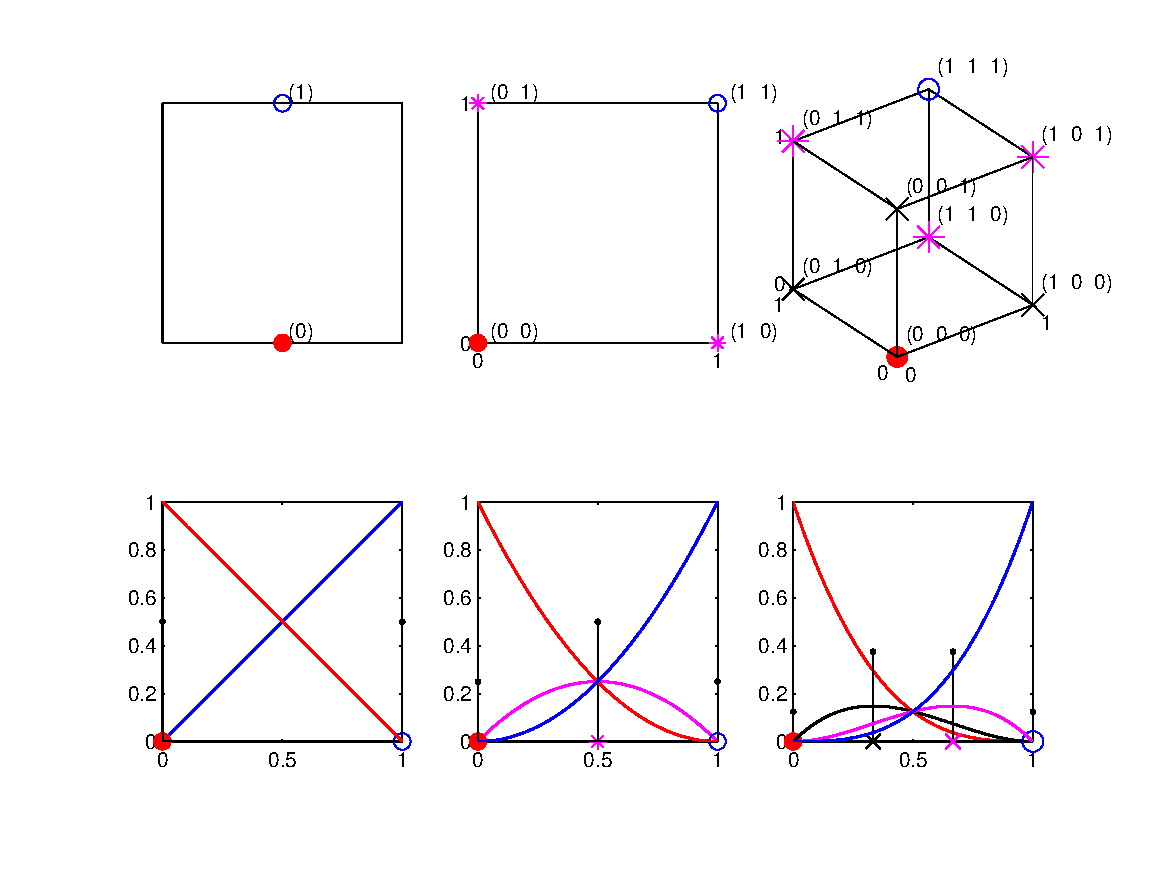
\includegraphics[width=5.0in]{figures/BernoulliSampleLkl}}
\end{figure}


\begin{definition}[Maximum Likelihood Estimator (MLE)]\label{D:MLE}
{\rm
Let the model for the data be
$$(X_1,\ldots,X_n) \sim f_{X_1,X_2,\ldots,X_n}(x_1,\ldots,x_n;\theta^*) \enspace .$$ 
Then the maximum likelihood estimator (MLE) $\widehat{\Theta}_n$ of the fixed and possibly unknown parameter $\theta^* \in \BB{\Theta}$ is the value of $\theta$ that maximizes the likelihood function:
\[
\boxed{
\widehat{\Theta}_n := \widehat{\Theta}_n(X_1,X_2,\ldots,X_n) :=  \argmax_{\theta \in \BB{\Theta}} L_n(\theta) \enspace ,
}
\]
Equivalently, MLE is the value of $\theta$ that maximizes the log-likelihood function (since $\log=\log_e=\ln$ is a monotone increasing function):
\[
\boxed{
\widehat{\Theta}_n := \argmax_{\theta \in \BB{\Theta}} \ell_n(\theta) \enspace ,
}
\]
}
\end{definition}

\subsubsection*{Useful Properties of the Maximum Likelihood Estimator}
\be
\item The ML Estimator is {\em asymptotically consistent} (gives the ``true'' $\theta^*$ as sample size $n \to \infty$):
\[
\boxed{\widehat{\Theta}_n \rightsquigarrow \pointmass(\theta^*)}
\]
\item The ML Estimator is asymptotically normal (has a normal distribution concentrating on $\theta^*$ as $n \to \infty$):
\[
\boxed{\widehat{\Theta}_n \rightsquigarrow \normal(\theta^*,(\widehat{\mathsf{se}}_n)^2)}
\]
or equivalently:
\[
\boxed{(\widehat{\Theta}_n - \theta^*) / \widehat{\mathsf{se}}_n \rightsquigarrow \normal(0,1)}
\]
where $\widehat{\mathsf{se}}_n$ is the {\bf estimated standard error}, i.e.~the standard deviation of $\widehat{\Theta}_n$, and it is given by the square-root of the inverse negative curvature of $\ell_n(\theta)$ at $\widehat{\theta}_n$:
\[
\boxed{
\widehat{\mathsf{se}}_n = \sqrt{\left( \left[ -\frac{d^2 \ell_n(\theta)}{d \theta^2}\right]_{\theta=\widehat{\theta}_n}\right)^{-1}}
}
\]
\item Because of the previous two properties, the $1-\alpha$ confidence interval is:
\[
\boxed{
\widehat{\Theta}_n \pm z_{\alpha/2} \widehat{\mathsf{se}}_n 
}
\]
%\item The ML Estimator is {\bf equivariant}, i.e.~$\widehat{\psi}_n=g(\widehat{\theta}_n)$ is the ML Estimate of $\psi^*=g(\theta^*)$, for some smooth function $g(\theta)=\psi: \BB{\Theta} \to \BB{\Psi}$.  
\ee

MLE is a general methodology for parameter estimation in an essentially arbitrary parameter space $\BB{\Theta}$ that is defining or indexing the laws in a parametric family of models, although we are only seeing it in action when $\BB{\Theta} \subset \Rz$ for simplest parametric family of models involving IID product experiments here.  
When $\BB{\Theta} \subset \Rz^d$ with $2 \leq d < \infty$ then MLE $\widehat{\Theta}_n \rightsquigarrow \pointmass(\theta^*)$, where $\theta^*=(\theta^*_1,\theta^*_2,\ldots,\theta^*_d)^{T}$ is a column vector in $\BB{\Theta} \subset \Rz^d$ 
and $\widehat{\Theta}_n \rightsquigarrow \normal\left(\theta^*,\widehat{\Sigma(\mathsf{se})}_n\right)$, a multivariate Normal distribution with mean vector $\theta^*$ and variance-covariance matrix of standard errors given by the {\em Hessian} (a $d \times d$ matrix of mixed partial derivatives) of $\ell_n(\theta_1,\theta_2,\ldots,\theta_d)$.  The ideas in the cased of dimension $d=1$ naturally generalize to an arbitrary, but finite, dimension $d$.
 
\begin{rem}
In order to use MLE for parameter estimation we need to ensure that the following two conditions hold:
\be
\item The {\em support} of the data, i.e.~the set of possible values of $(X_1,X_2,\ldots,X_n)$ must not depend on $\theta$ for every $\theta \in \BB{\Theta}$ --- of course the probabilities do depend on $\theta$ in an {\em identifiable} manner, i.e.~for every $\theta$ and $\vartheta$ in $\BB{\Theta}$, if $\theta \neq \vartheta$ then $f_{X_1,X_2,\ldots,X_n}(x_1,x_2,\ldots,x_n;\theta) \neq f_{X_1,\ldots,X_n}(x_1,x_2,\ldots,x_n;\vartheta)$ at least for some $(x_1,x_2,\ldots,x_n) \in \Xz$.
\item If the parameter space $\BB{\Theta}$ is bounded then $\theta^*$ must not belong to the boundaries of $\BB{\Theta}$.
\ee
\end{rem}

\subsubsection*{Maximum Likelihood Estimation Method in Six Easy Steps}
{\bf Background:} We have observed data:
\[
(x_1,x_2,\ldots,x_n)
\]
which is modeled as a sample or realization from the random vector:
\[
(X_1,X_2,\ldots,X_n) \sim f_{X_1,X_2,\ldots,X_n}(x_1,x_2,\ldots,x_n; \theta^*), \quad \theta^* \in \BB{\Theta} \enspace .
\]
{\bf Objective:} We want to obtain an estimator $\widehat{\Theta}_n$ that will give:
\be
\item the point estimate $\widehat{\theta}_n$ of the ``true'' parameter $\theta^*$ and
\item the $(1-\alpha)$ confidence interval for $\theta^*$.
\ee
{\bf Steps of MLE:} 
\begin{itemize}
\item{{\sf Step 1}:} Find the expression for the log likelihood function:
\[
\ell_n(\theta) = \log(L_n(\theta)) = \log\left( f_{X_1,X_2,\ldots,X_n}(x_1,x_2,\ldots,x_n; \theta) \right) \enspace .
\]
Note that if the model assumes that $(X_1,X_2,\ldots,X_n)$ is jointly independent, i.e.~we have an independent and identically distributed (IID) experiment, then $\ell_n(\theta)$ simplifies further as follows:
\[
\ell_n(\theta) = \log(L_n(\theta)) = \log\left( f_{X_1,X_2,\ldots,X_n}(x_1,x_2,\ldots,x_n; \theta) \right) = \log \left(\prod_{i=1}^n f_{X_i}(x_i;\theta) \right) %= \sum_{i=1}^n \log\left(f_{X_i}(x_i;\theta)\right) 
\enspace .
\]

\item{{\sf Step 2}:} Obtain the derivative of $\ell_n(\theta)$ with respect to $\theta$:
\[
\frac{d}{d \theta}\left(\ell_n(\theta)\right) \enspace .
\]
\item{{\sf Step 3}:} Set the derivative equal to zero, solve for $\theta$ and let $\widehat{\theta}_n$ equal to this solution. 
\item{{\sf Step 4}:} Check if this solution is indeed a maximum of $\ell_n(\theta)$ by checking  if:
\[
\frac{d^2}{d \theta^2}\left(\ell_n(\theta)\right) < 0 \enspace .
\]
\item{{\sf Step 5}:} If $\frac{d^2}{d \theta^2}\left(\ell_n(\theta)\right) < 0$ then you have found the maximum likelihood estimate $\widehat{\theta}_n$.
\item{{\sf Step 6}:} If you also want the $(1-\alpha)$ confidence interval then get it from
\[
\widehat{\theta}_n \pm z_{\alpha/2} \widehat{\mathsf{se}}_n \quad \text{, where } \quad \widehat{\mathsf{se}}_n = \sqrt{\left( \left[ -\frac{d^2 \ell_n(\theta)}{d \theta^2}\right]_{\theta=\widehat{\theta}_n}\right)^{-1}} \enspace .
\]
\end{itemize}

Let us apply this method in some examples.

\remove{
\Exmp{
\label{Eg:ExponentialMLE}
Find (or derive) the maximum likelihood estimate $\widehat{\lambda}_n$ and the $(1-\alpha)$ confidence interval of the fixed and possibly unknown parameter $\lambda^*$ for the IID experiment:
$$X_1,\ldots,X_n \overset{IID}{\sim} \exponential(\lambda^*), \qquad \lambda^* \in \BB{\Lambda} = (0,\infty) \enspace .$$
Note that $\BB{\Lambda}$ is the parameter space.

We first obtain the log-likelihood function $\ell_n(\theta)$ given data $(x_1,x_2,\ldots,x_n)$.
\begin{flalign*}
\ell_n(\lambda) 
& := \log(L(x_1,x_2,\ldots,x_n;\lambda))  = \log \left( \prod_{i=1}^n f_{X_i}(x_i;\lambda) \right) = \log \left( \prod_{i=1}^n \lambda e^{-\lambda x_i}  \right)\\
& = \log \left( \lambda e^{-\lambda x_1} \cdot \lambda e^{-\lambda x_2}  \cdots \lambda e^{-\lambda x_n}  \right) = \log \left( \lambda^n e^{-\lambda \sum_{i=1}^n x_i}  \right) =\log \left( \lambda^n \right) + \log \left( e^{-\lambda \sum_{i=1}^n x_i}  \right) \\
&= \boxed{\log \left( \lambda^n \right) -\lambda \sum_{i=1}^n x_i}
\end{flalign*}

Now, let us take the derivative with respect to $\lambda$,
\begin{flalign*}
\frac{d}{d \lambda} \left( \ell_n(\lambda) \right) 
& :=  \frac{d}{d \lambda} \left( 
\log \left( \lambda^n \right) -\lambda \sum_{i=1}^n x_i
\right) = \frac{d}{d \lambda} \left( 
\log \left( \lambda^n \right) \right) -  \frac{d}{d \lambda} \left( \lambda \sum_{i=1}^n x_i \right)  = \frac{1}{\lambda^n}  \frac{d}{d \lambda} \left( \lambda^n \right) - \sum_{i=1}^n x_i \\
&= \frac{1}{\lambda^n}  n \lambda^{n-1}  - \sum_{i=1}^n x_i = \boxed{\frac{n}{\lambda} - \sum_{i=1}^n x_i } \enspace .
\end{flalign*}
Next, we set the derivative to $0$, solve for $\lambda$, and let the solution equal to the ML estimate $\widehat{\lambda}_n$.
\begin{flalign*}
0 = \frac{d}{d \lambda} \left( \ell_n(\lambda) \right) 
& \iff 0 = \frac{n}{\lambda} - \sum_{i=1}^n x_i \iff \sum_{i=1}^n x_i = \frac{n}{\lambda} \iff \lambda = \frac{n}{\sum_{i=1}^n x_i} \quad \text{ and let } \boxed{\widehat{\lambda}_n = \frac{1}{\overline{x}_n}} \enspace .
\end{flalign*}
Next, we find the second derivative and check if it is negative.
\begin{flalign*}
\frac{d^2}{d \lambda^2} \left( \ell_n(\lambda) \right) 
&= \frac{d}{d \lambda} \left( \frac{d}{d \lambda} \left( \ell_n(\lambda) \right) \right) = \frac{d}{d \lambda} \left( \frac{n}{\lambda} - \sum_{i=1}^n x_i \right) = \boxed{-n\lambda^{-2}} \enspace .
\end{flalign*}
Since $\lambda>0$ and $n \in \Nz$, $\boxed{-n\lambda^{-2}=-n/\lambda^2 < 0}$, so we have found the maximum likelihood estimate:
\[
\boxed{\widehat{\lambda}_n = \frac{1}{\overline{x}_n} } \enspace .
\]
Now, let us find the estimated standard error:
\begin{align*}
\boxed{\widehat{\mathsf{se}}_n} 
&= \sqrt{\left( \left[ -\frac{d^2 \ell_n(\lambda)}{d \lambda^2}\right]_{\lambda=\widehat{\lambda}_n}\right)^{-1}} 
= \sqrt{\left( \left[ - \left( -\frac{n}{\lambda^2}\right) \right]_{\lambda=\widehat{\lambda}_n}\right)^{-1}} = \sqrt{\left( \frac{n}{\widehat{\lambda}_n^2}\right)^{-1}}=\sqrt{\frac{\widehat{\lambda}_n^2}{n}}=\frac{\widehat{\lambda}_n}{\sqrt{n}}\\
&=\boxed{\frac{1}{\ol{x}_n\sqrt{n}}}
\enspace .
\end{align*}
And finally, the $(1-\alpha)$ confidence interval is
\[
\widehat{\lambda}_n \pm z_{\alpha/2} \widehat{\mathsf{se}}_n 
= \boxed{\frac{1}{\overline{x}_n} \pm z_{\alpha/2} \frac{1}{\ol{x}_n\sqrt{n}}} \enspace . 
\]
}

Since we have worked ``hard'' to get the maximum likelihood estimate for a general IID model $X_1,X_2,\ldots,X_n \overset{IID}{\sim} \exponential(\lambda^*)$.  Let us kill two birds with the same stone by applying it to two datasets:
\be
\item Orbiter waiting times and
\item Time between measurable earthquakes in New Zealand over a few months.
\ee


Therefore, the ML estimate $\widehat{\lambda}_n$ of the unknown rate parameter $\lambda^* \in \BB{\Lambda}$ on the basis of $n$ IID observations $x_1,x_2,\ldots,x_n \overset{IID}{\sim} \exponential(\lambda^*)$ is $1/\overline{x}_n$ and the ML estimator $\widehat{\Lambda}_n=1/\overline{X}_n$.  Let us apply this ML estimator of the rate parameter for the supposedly exponentially distributed waiting times at the on-campus Orbiter bus-stop.

%\begin{VrbM}
%% Joshu Fenemore’s Data from 2007 on Waiting Times at Orbiter Bust Stop by Balgay Street
%%The raw data -- the waiting times to nearest minute between Orbiter buses
%>> orbiterTimes=[8 3 7 18 18 3 7 9 9 25 0 0 25 6 10 0 10 8 16 9 1 5 16 6 4 1 3 21 0 28 3 8 ...
% 6 6 11 8 10 15 0 8 7 11 10 9 12 13 8 10 11 8 7 11 5 9 11 14 13 5 8 9 12 10 13 6 11 13 ...
% 0 0 11 1 9 5 14 16 2 10 21 1 14 2 10 24 6 1 14 14 0 14 4 11 15 0 10 2 13 2 22 ...
% 10 5 6 13 1 13 10 11 4 7 9 12 8 16 15 14 5 10 12 9 8 0 5 13 13 6 8 4 13 15 7 11 6 23 1];
%>> mean(orbiterTimes)
%ans =
%    9.0758
%\end{VrbM}

{\bf Orbiter Waiting Times}

Joshua Fenemore and Yiran Wang collected data on waiting times between buses at an Orbiter bus-stop close to campus.  
They collected a sample of size $n=132$ with sample mean $\overline{x}_{132}=9.0758$.
From our work in Example~\ref{Eg:ExponentialMLE} we can now easily obtain the maximum likelihood estimate of $\lambda^*$ and the $95\%$ confidence interval for it, under the assumption that the waiting times $X_1,\ldots,X_{132}$ are IID $\exponential(\lambda^*)$ RVs as follows: 
$$\widehat{\lambda}_{132}=1/\overline{x}_{132}=1/9.0758=0.1102 \quad 
(0.1102 \pm 1.96 \times 0.1102/\sqrt{132}) = (0.0914,0.1290) \enspace ,$$ 
and thus the estimated mean waiting time is 
$$1/\widehat{\lambda}_{132}=9.0763 \text{ minutes} .$$  
The estimated mean waiting time for a bus to arrive is well within the $10$ minutes promised by the Orbiter bus company.  
This data and its maximum likelihood analysis is presented visually in Figure~\ref{F:ExponentialMLEOrbiter}.
 
%The following script was used to generate the \hyperref[F:ExponentialMLE]{Figure \ref*{F:ExponentialMLEOrbiter}}:
\begin{figure}[htpb]
\caption{Plot of $\log(L(\lambda))$ as a function of the parameter $\lambda$  and the MLE $\widehat{\lambda}_{132}$ of $0.1102$ for Fenemore-Wang Orbiter Waiting Times Experiment from STAT 218 S2 2007.  The density or PDF and the DF at the MLE of $0.1102$ are compared with a histogram and the empirical DF.\label{F:ExponentialMLEOrbiter}}
\centering   \makebox{\includegraphics[width=4.5in]{../../../figures/ExponentialMLEOrbiter}}
\end{figure}
Notice how the exponential PDF $f(x;\widehat{\lambda}_{132}=0.1102)$ and the DF $F(x;\widehat{\lambda}_{132}=0.1102)$ based on the MLE fits with the histogram and the empirical DF, respectively.  
%This is an indication of the inadequacy of our parametric model.  Partly this discrepancy is due to the resolution of the the measurements being confined to whole minutes.  We can overcome this problem by fitting a minute-discretized PMF from the $\exponential(\lambda)$ PDF.  

\begin{figure}[htpb]
\caption{Comparing the $\exponential(\widehat{\lambda}_{6128}= 28.6694)$ PDF and DF with a histogram and empirical DF of the times (in units of days) between earth quakes in  NZ.  The epicenters of $6128$ earth quakes are shown in left panel.\label{F:NZSIEarthQuakesExponentialMLE}}
\centering   \makebox{\includegraphics[width=4.5in]{../../../figures/NZSIEarthQuakesExponentialMLE}}
\end{figure}

{\bf Waiting Times between Earth Quakes in NZ:}%\label{LW:NZSIEarthQuakesExponentialMLE}  

Once again from our work in Example~\ref{Eg:ExponentialMLE} we can now easily obtain the maximum likelihood estimate of $\lambda^*$ and the $95\%$ confidence interval for it, under the assumption that the waiting times (in days) between the $6128$ measurable earth-quakes in NZ from 18-Jan-2008 02:23:44 to 18-Aug-2008 19:29:29 are IID $\exponential(\lambda^*)$ RVs as follows: 
$$\widehat{\lambda}_{6128}=1/\overline{x}_{6128}=1/0.0349=28.6694 \quad 
(28.6694 \pm 1.96 \times 28.6694/\sqrt{6128}) = (27.95,29.39) \enspace ,$$ 
and thus the estimated mean time in days and minutes between earth quakes (somewhere in NZ over the first 8 months in 2008) is 
$$1/\widehat{\lambda}_{6128}=\overline{x}_{6128}=0.0349 \text{ days } \quad = \quad 0.0349*24*60=50.2560  \text{ minutes} \enspace .$$  
This data and its maximum likelihood analysis is presented visually in Figure~\ref{F:NZSIEarthQuakesExponentialMLE}.  The PDF and DF corresponding to the $\widehat{\lambda}_{6128}$ (blue curves in Figure~\ref{F:NZSIEarthQuakesExponentialMLE}) are the best fitting PDF and DF from the parametric family of PDFs in $\{\lambda e^{-\lambda x}: \lambda \in (0,\infty) \}$ and DFs in $\{1- e^{-\lambda x}: \lambda \in (0,\infty) \}$ to the density histogram and the empirical distribution function given by the data, respectively.  Clearly, there is room for improving beyond the model of IID $\exponential(\lambda)$ RVs, but the fit with just one real-valued parameter is not too bad either.  Finally, with the best fitting PDF $28.6694 e^{-28.6694 x}$ we can get probabilities of events and answer questions like: ``what is the probability that there will be three earth quakes somewhere in NZ within the next hour?'', etc.

%as computed in the following script:\VrbMf[label=NZSIEarthQuakesExponentialMLE.m]{../../../scripts/NZSIEarthQuakesExponentialMLE.m}
%We first load the data in the text file {\tt earthquakes.csv} into a matrix {\tt EQ}.  Using the {\tt datenum} function in {\sc Matlab} we transform the time stamps into a number starting at zero.  These transformed time stamps are in units of days.  Then we find the times between consecutive events and estimate a histogram.  We finally compute the ML estimate of $\lambda^*$ and super-impose the PDF of the $\exponential(\widehat{\lambda}_{6128}= 28.6694)$ upon the histogram.
%\begin{VrbM}
%>> NZSIEarthQuakesExponentialMLE
%ans =        6128          13
%
%Earth Quakes in NZ between
%18-Jan-2008 02:23:44 and18-Aug-2008 19:29:29
%
%SampleMean =    0.0349
%MLELambdaHat =   28.6694
%\end{VrbM}
%Thus, the average time between earth quakes is $0.0349*24*60=50.2560$ minutes.
%\end{labwork}

\begin{example}[ML Estimation for the IID $\bernoulli(\theta^*)$ experiment]\label{EX:MLECoinTossing}
{\rm 
Let us do maximum likelihood estimation for the coin-tossing experiment of Example~\ref{EX:CoinTossing} with likelihood derived in Example~\ref{EX:LklCoinTossing} to obtain the maximum likelihood estimate $\widehat{\theta}_n$ of the unknown parameter $\theta^* \in \BB{\Theta} = [0,1]$ and the $(1-\alpha)$ confidence interval for it.

From Equation~\eqref{E:LklBernoulli} the log likelihood function is
\begin{eqnarray}
\ell_n(\theta) = \log(L_n(\theta)) 
= \log \left( \theta^{\sum_{i=1}^n x_i} (1-\theta)^ {n-\sum_{i=1}^n x_i} \right) 
= \boxed{\left({\sum_{i=1}^n x_i}\right) \log(\theta) + \left(n-{\sum_{i=1}^n x_i}\right) \log(1-\theta)} \notag \enspace ,
\end{eqnarray}
Next, we take the derivative with respect to the parameter $\theta$:
\begin{eqnarray}
\frac{d}{d \theta} \left(\ell_n(\theta)\right) 
&=& \frac{d}{d \theta}  \left( \left({\sum_{i=1}^n x_i}\right) \log(\theta) \right) + \frac{d}{d \theta} \left(  \left( n-{\sum_{i=1}^n x_i} \right) \log(1-\theta) \right) \notag = \boxed{\frac{{\sum_{i=1}^n x_i}}{\theta} - \frac{n-{\sum_{i=1}^n x_i}}{1-\theta}} \notag \enspace .
\end{eqnarray}
Now, set $\frac{d}{d \theta} \log(L_n(\theta))=0$, solve for $\theta$ and set the solution equal to $\widehat{\theta}_n$: 
\begin{align*}
\frac{d}{d \theta} \left( \ell_n(\theta) \right) = 0 
&\iff  \frac{{\sum_{i=1}^n x_i}}{\theta} = \frac{n-{\sum_{i=1}^n x_i}}{1-\theta} \iff
\frac{1-\theta}{\theta} = \frac{n-{\sum_{i=1}^n x_i}}{{\sum_{i=1}^n x_i}} \\
&\iff
\frac{1}{\theta}-1 = \frac{n}{{\sum_{i=1}^n x_i}}-1 \quad \text{ let } \boxed{\widehat{\theta}_n = \frac{{\sum_{i=1}^n x_i}}{n}}
\end{align*}
Next, we find the second derivative and check if it is negative.
\begin{align*}
\frac{d^2}{d \theta^2} (\ell_n(\theta)) 
&= \frac{d}{d \theta} \left( \frac{{\sum_{i=1}^n x_i}}{\theta} - \frac{n-{\sum_{i=1}^n x_i}}{1-\theta} \right) 
= \boxed{-\frac{{\sum_{i=1}^n x_i}}{\theta^2} - \frac{n-{\sum_{i=1}^n x_i}}{(1-\theta)^2}} 
\end{align*}

Since each term in the numerator and the denominator of the two fractions in the above box are non-negative, $\frac{d^2}{d \theta^2} (\ell_n(\theta))< 0$ and therefore we have found the maximum likelihood estimate
\[
\widehat{\theta}_n  = \frac{1}{n} \sum_{i=1}^n x_i = \overline{x}_n
\]
We already knew this to be a point estimate for $E(X_i)=\theta^*$ from LLN and CLT.  But now we know that MLE also agrees.
Now, let us find the estimated standard error:
\begin{align*}
\boxed{\widehat{\mathsf{se}}_n} 
&= \sqrt{\left( \left[ -\frac{d^2 \ell_n(\theta)}{d \theta^2}\right]_{\theta=\widehat{\theta}_n}\right)^{-1}} 
= \sqrt{\left( \left[ - \left( -\frac{{\sum_{i=1}^n x_i}}{\theta^2} - \frac{n-{\sum_{i=1}^n x_i}}{(1-\theta)^2}\right) \right]_{\theta=\widehat{\theta}_n}\right)^{-1}} \\
&= \sqrt{\left( \frac{{\sum_{i=1}^n x_i}}{\widehat{\theta}_n^2} + \frac{n-{\sum_{i=1}^n x_i}}{(1-\widehat{\theta}_n)^2} \right)^{-1}}
= \sqrt{\left( \frac{n\ol{x}_n}{\ol{x}_n^2} + \frac{n-n\ol{x}_n}{(1-\ol{x}_n)^2} \right)^{-1}}
= \sqrt{\left( \frac{n}{\ol{x}_n} + \frac{n}{(1-\ol{x}_n)} \right)^{-1}}\\
&= \sqrt{\left( \frac{n(1-\ol{x}_n)+n\ol{x}_n}{\ol{x}_n(1-\ol{x}_n)} \right)^{-1}}
= \sqrt{\frac{\ol{x}_n(1-\ol{x}_n)}{n((1-\ol{x}_n)+\ol{x}_n}}
= \boxed{\sqrt{\frac{\ol{x}_n(1-\ol{x}_n)}{n}}} \enspace .\\
\enspace .
\end{align*}
And finally, the $(1-\alpha)$ confidence interval is
\[
\widehat{\theta}_n \pm z_{\alpha/2} \widehat{\mathsf{se}}_n 
= \boxed{\overline{x}_n \pm z_{\alpha/2} \sqrt{\frac{\ol{x}_n(1-\ol{x}_n)}{n}}} \enspace . 
\]

For the coin tossing experiment that was performed ($n=10$ times) in Example~\ref{EX:CoinTossing}, the maximum likelihood estimate of $\theta^*$ and the $95\%$ confidence interval for it, under the model that the tosses are IID $\bernoulli(\theta^*)$ RVs, are as follows:
\[
\widehat{\theta}_{10} 
= \ol{x}_{10} =\frac{4}{10}=0.40
\quad \text{and} \quad \left(0.4 \pm 1.96 \times \sqrt{\frac{0.4 \times 0.6}{10}}\right) =  (0.0964, 0.7036) \enspace .
\]
See Figures~\ref{F:BernoulliMLE} and \ref{F:BernoulliMLEConsistency} to completely understand parameter estimation for IID Bernoulli experiments.
% (not just coin toss, but for any event of interest!) through the pictures.
}
\end{example}

\begin{figure}[htpb]
\caption{Plots of the log likelihood $\ell_n(\theta)=\log(L(1,0,0,0,1,1,0,0,1,0;\theta))$ as a function of the parameter $\theta$ over the parameter space $\BB{\Theta}=[0,1]$ and the MLE $\widehat{\theta}_{10}$ of $0.4$ for the coin-tossing experiment shown in standard scale (left panel) and log scale for $x$-axis (right panel).\label{F:BernoulliMLE}}
\centering   \makebox{\includegraphics[width=5.5in]{../../../figures/BernoulliMLE}}
\end{figure}


\begin{figure}[htbp]
\caption{{\small $100$ realizations of $95\%$ confidence intervals based on samples of size $n$ $=$ $10$, $100$ and $1000$ simulated from IID $\bernoulli(\theta^*=0.5)$ RVs.  %as per \hyperref[Mf:BernoulliMLEConsistency]{Labwork~\ref*{Mf:BernoulliMLEConsistency}}.  
The MLE $\widehat{\theta}_n$ (cyan dot) and the log-likelihood function (magenta curve) for each of the $100$ replications of the experiment for each sample size $n$ are depicted.  
The approximate normal-based $95\%$ confidence intervals with blue boundaries are based on the exact $\mathsf{se}_n=\sqrt{\theta^*(1-\theta^*)/n}=\sqrt{1/4}$, while those with red boundaries are based on the estimated $\widehat{\mathsf{se}_n}=\sqrt{\widehat{\theta}_n(1-\widehat{\theta}_n)/n} = \sqrt{\frac{\ol{x}_n(1-\ol{x}_n)}{n}}$.  
The fraction of times the true parameter $\theta^*=0.5$ was contained by the exact and approximate confidence interval (known as {\em empirical coverage}) over the $100$ replications of the simulation experiment for each of the three sample sizes are given by the numbers after {\tt Cvrg.=} and {\tt $\sim$=}, above each sub-plot, respectively.}\label{F:BernoulliMLEConsistency}}
\begin{center}
\makebox{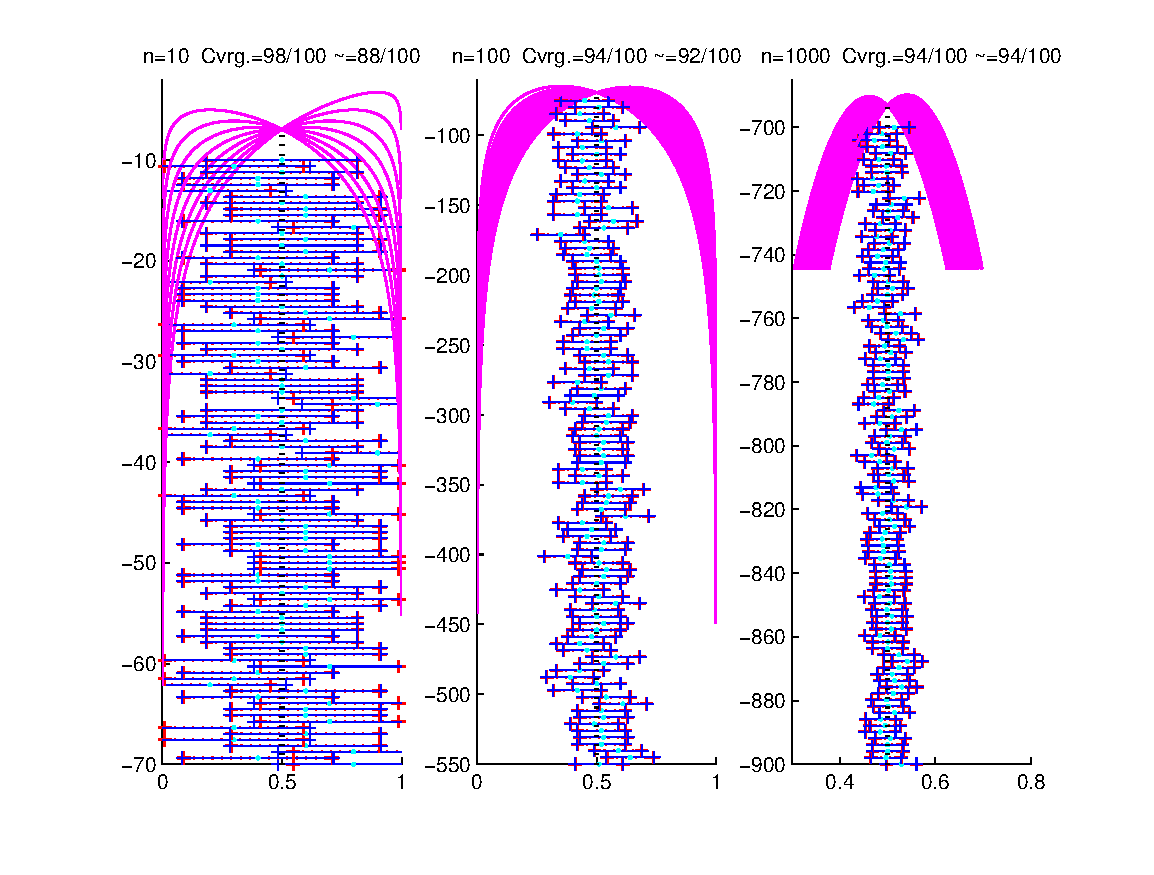
\includegraphics[width=6.00in]{../../../figures/BernoulliMLEConsistency}}
\end{center}
\end{figure}  

\clearpage

\iftoggle{PlaceTutsHere}{%
\subsection{Tutorial Exercises}
\input{Tutorials/Tut_Lkl_preps.tex}
~\\
\input{Tutorials/Tut_Lkl_inTut.tex}
}{%
  % don't do anything otherwise
}

%%%%%%%%%%%%%%%%%%%%%%%%%%%%%%%%%%%%%%%%%%%%%%%%%%%%%%%%%%%%%%%%%%%%%%%%%%%%%%%%%%%%%%%%%%%%%


%Sorry ---  no time to make an exhaustive glossary of all the notation yet. 
%\subsubsection*{Summarizing Table of Point Estimators}
%Using the sample mean $\overline{X}_n$ and sample standard deviation $S_n$ defined in \eqref{E:SampleMeanRV} and \eqref{E:SampleStdDevRV}, respectively, we summarise the two point estimators of the parameters of some common distributions below.  For some cases, the MLE is the same as the MME and can be solved analytically.
%\begin{center}
%\begin{table}[htbp]
%\caption{Summary of the Method of Moment Estimator (MME) and the Maximum Likelihood Estimator (MLE) for some IID Experiments. \label{T:MMEMLE}}
%\begin{tabular}{l | r | r}
%\hline
%Statistical Experiment & MLE & MME \\ \hline
%$X_1,X_2,\ldots,X_n \overset{IID}{\sim} \bernoulli(\theta)$ & $\widehat{\theta}=\overline{X}_n$ & same as MLE \\ \hline
%$X_1,X_2,\ldots,X_n \overset{IID}{\sim} \exponential(\lambda)$ & $\widehat{\lambda}={1}/{\overline{X}_n} $ & same as MLE \\ \hline
%$X_1,X_2,\ldots,X_n \overset{IID}{\sim} \normal(\mu,\sigma^2)$ & $\widehat{\mu}=\overline{X}_n, \widehat{\sigma} = \sqrt{\frac{n-1}{n}S^2_n} $ & $\widehat{\mu}=\overline{X}_n, \widehat{\sigma} = S_n $ \\ \hline
%$X_1,X_2,\ldots,X_n \overset{IID}{\sim} \lognormal(\lambda,\zeta)$ & $\widehat{\lambda}=\frac{1}{n}{\sum_{i=1}^n \log(X_i)} $ & $\widehat{\lambda} = \log(\overline{X}_n) - \frac{1}{2} {\widehat{\zeta}} \ ^2$ \\ %\\
% & $\widehat{\zeta} = \sqrt{\frac{1}{n} \sum_{i=1}^n{(\log(X_i)-\widehat{\lambda})^2}} $ & $\widehat{\zeta} = \sqrt{\log \left({S_n^2}/{\overline{X}_n^2} +1 \right)}$ \\
%\hline
%\end{tabular}
%\end{table}
%\end{center}


%\begin{labwork}
%Choose some parameter $p\in[0,1]$ and some sample size $n$.  Then, using the {\sc Matlab} expression {\tt floor(rand(1,n)+p)} (See \hyperref[SIM:Bernoulli]{Simulation~\ref*{SIM:Bernoulli}}) simulate $n$ IID $\bernoulli(p)$ RVs $X_1,X_2,\ldots,X_n$.  Once you have generated the data, pretend that you don't know the $p$ used in your simulation and estimate $p$ using the sample mean estimator we have seen in \hyperref[EX:EstimatePFromNIIDBernoulliTrials]{Example~\ref*{EX:EstimatePFromNIIDBernoulliTrials}},  That is, compute the estimate $\widehat{p}_n=n^{-1}\sum_{i=1}^n x_i$ and also the approximate $95\%$ Normal-based confidence interval $C_n = \widehat{p}_n \pm 1.96 \sqrt{\frac{\widehat{p}_n(1-\widehat{p}_n)}{n}}$.

%For each value of $p \in [0, 1/100, 1/10, 2/10, 3/10, 4/10, 5/10, 6/10, 7/10, 8/10, 9/10, 9/100, 1]$,  generate $n$ IID $\bernoulli(p)$ samples where $n$ ranges in $\{10^i: i =1,2,3,4,5 \}$ and estimate $p$ from the simulated data of different sample sizes.  Do you intuitively agree with the behavior of the confidence intervals, in terms of the changes in their widths, as $n$ gets large for each of the fixed $p$'s ?  Is the point estimate $\widehat{p}_n$ approaching the $p$ from which the data were simulated for each of the fixed $p$'s as $n$ gets large ?
%For each value of $p$ as before, generate, say $1000$ data sets each of sample size $n \in \{10^i: i =1,2,3,4,5 \}$ and empirically study the coverage properties of the estimator.  That is, for each $p$ and $n$, find what fraction of the Normal-based  $95\%$ confidence intervals constructed from each of the $1000$ replicate data sets actually contain the parameter $p$ that they were simulated from.  Try to explain why coverage properties are both a function of how close $p$ is to the boundary of the the parameter space $[0,1]$ and the sample size $n$.  [Inspired by Russell Gribble]
%\end{labwork}

}


%\section{Moment Estimator (MME)}\label{S:MME}
%See notes from class.  

%original cse book notes to be reabsorbed into the condensed content above
\remove{
\chapter{Maximum Likelihood Estimator}

Next we look at a specific point estimator called the maximum likelihood estimator (MLE) of a possibly unknown but fixed parameter $\theta^*$ in a parametric experiment, i.e.~$\theta^* \in \BB{\Theta} \subset \Rz^k$ with $k < \infty$.  Other point estimators in such a setting include the moment estimator (MME). 

Recall that the likelihood function (See \hyperref[D:LklFn]{Definition~\ref*{D:LklFn}}) for an IID experiment with observations $x_1,x_2,\ldots,x_n$ is simply the product of the densities:
$$L_n(\theta)=\prod_{i=1}^n f(x_i;\theta) : \BB{\Theta} \to (0,\infty) \enspace , $$
and its logarithm or log-likelihood function is:
$$\ell_n(\theta)= \log(L_n(\theta)) = \sum_{i=1}^n \log(f(x_i)) :  \BB{\Theta} \to (-\infty,\infty) \enspace . $$

\section{Introduction to Maximum Likelihood Estimation}\label{S:MLE}
\begin{definition}[Maximum Likelihood Estimator (MLE)]\label{D:MLE}
Let $X_1,\ldots,X_n \sim f(x_1,\ldots,x_n;\theta^*)$.  The maximum likelihood estimator (MLE) $\widehat{\Theta}_n$ of the fixed and possibly unknown parameter $\theta^* \in \BB{\Theta}$ is the value of $\theta$ that maximises the likelihood function:
\[
\boxed{
\widehat{\Theta}_n := \widehat{\Theta}_n(X_1,X_2,\ldots,X_n) :=  \argmax_{\theta \in \BB{\Theta}} L_n(\theta) \enspace ,
}
\]
Equivalently, MLE is the value of $\theta$ that maximises the log-likelihood function:
\[
\boxed{
\widehat{\Theta}_n := \argmax_{\theta \in \BB{\Theta}} \ell_n(\theta) \enspace ,
}
\]
since the maximum of the likelihood coincides with that of the log-likelihood.  It is analytically and numerically convenient to work with the log-likelihood instead of the likelihood.  Optimisation algorithms can be used to find the MLE numerically.  Such algorithms by convention tend to find the minimum and the value that minimises a function.  So, the MLE is also the the value of $\theta$ that minimises the negative likelihood or negative log-likelihood functions:
\[
\boxed{
\widehat{\Theta}_n := \argmin_{\theta \in \BB{\Theta}} -L_n(\theta), \qquad
\widehat{\Theta}_n := \argmin_{\theta \in \BB{\Theta}} -\ell_n(\theta)  \enspace .
}
\]
Once again, the realisation of the MLE, namely $\widehat{\theta}_n = \widehat{\Theta_n}(x_1,\ldots,x_n)$ based on the observation is the maximum likelihood estimate (MLe) of the $\theta^*$.
\end{definition}

\begin{example}[Coin Tossing Experiment ($X_1,\ldots,X_{10} \overset{IID}{\sim} \bernoulli(\theta^*)$)]\label{EX:CoinTossingML}
I tossed a coin that has an unknown probability $\theta^*$ of landing Heads independently and identically $10$ times in a row.  Four of my outcomes were Heads and the remaining six were Tails, with the actual sequence of Bernoulli outcomes (Heads $\to 1$ and Tails $\to 0$) being $(1,0,0,0,1,1,0,0,1,0)$.  I would like to estimate the probability $\theta^* \in \BB{\Theta} = [0,1]$ of observing Heads using the maximum likelihood estimator or MLE $\widehat{\Theta}_n((X_1,X_2,\ldots,X_n))$ of $\theta$. We derive the MLE next.

First, the likelihood function is:
\begin{eqnarray}
L_n(\theta) &:=& L_n(x_1,x_2,\ldots,x_n; \theta)  =  \prod_{i=1}^n f(x_i|\theta) = \theta^{\sum_{i=1}^n x_i} (1-\theta)^ {n-\sum_{i=1}^n x_i} := \theta^{t_n} (1-\theta)^{n-t_n} \notag 
\end{eqnarray}
In the last step, we have formally defined the following statistic of the data: 
$$T_n(X_1,X_2,\ldots,X_n)=\sum_{i=1}^n X_i :  \Xz_n \rightarrow \Tz_n$$ with the corresponding realisation $t_n := T_n(x_1,x_2,\ldots,x_n)=\sum_{i=1}^n x_i \in \Tz_n$.  Let us now take the natural logarithm of both sides:
\begin{eqnarray}
\log(L_n(\theta)) := \log(L(x_1,x_2,\ldots,x_n; \theta))   
= \log \left( \theta^{t_n} (1-\theta)^ {n-t_n} \right) 
= t_n \log(\theta) + (n-t_n) \log(1-\theta) \notag
\end{eqnarray}
Next, we take the derivative with respect to the parameter $\theta$:
\begin{eqnarray}
\frac{\partial}{\partial \theta} \log(L_n(\theta)) 
&=& \frac{\partial}{\partial \theta}  t_n \log(\theta) + \frac{\partial}{\partial \theta}  (n-t_n) \log(1-\theta) \notag \\
&=& \frac{t_n}{\theta} - \frac{n-t_n}{1-\theta} \notag
\end{eqnarray}
Now, set $\frac{\partial}{\partial \theta} \log(L_n(\theta))=0$ and solve for $\theta$ to obtain the maximum likelihood estimate  $\widehat{\theta}_n$:
\[
\frac{\partial}{\partial \theta} \log(L(\theta)) = 0 \iff  
\frac{t_n}{\theta} = \frac{n-t_n}{1-\theta} \iff
\frac{1-\theta}{\theta} = \frac{n-t_n}{t_n} \iff
\frac{1}{\theta}-1 = \frac{n}{t_n}-1 \iff \widehat{\theta}_n = \frac{t_n}{n}
\]
Therefore the MLE is:
\[
\widehat{\Theta}_n(X_1,X_2,\ldots,X_n) = \frac{1}{n}T_n(X_1,X_2,\ldots,X_n) = \frac{1}{n} \sum_{i=1}^n X_i = \overline{X}_n
\]
For the coin tossing experiment I just performed ($n=10$ times), the point estimate of $\theta$ is:
\begin{eqnarray}
\widehat{\theta}_{10} = \widehat{\Theta}_{10}((x_1,x_2,\ldots,x_{10})) 
&=&\widehat{\Theta}_{10}((1,0,0,0,1,1,0,0,1,0)) \notag \\
&=& \frac{1+0+0+0+1+1+0+0+1+0}{10}=\frac{4}{10}=0.40 \notag \ .
\end{eqnarray}
\end{example}

\section{Practical Excursion in One-dimensional Optimisation}
Numerically maximising a log-likelihood function of one parameter is a useful technique.  This can be used for models with no analytically known MLE.  A fairly large field of maths, called optimisation, exists for this sole purpose.  Conventionally, in optimisation, one is interested in minimisation.  Therefore, the basic algorithms are cast in the ``find the minimiser and the minimum'' of a target function $f:\Rz \to \Rz$.  Since we are interested in maximising our target, which is the likelihood or log-likelihood function, say $\log(L(x_1,\ldots,x_n; \theta)): \BB{\Theta} \to \Rz$, we will simply apply the standard optimisation algorithms directly to $-\log(L(x_1,\ldots,x_n; \theta)):\BB{\Theta}\to \Rz$.

The algorithm implemented in {\tt fminbnd} is based on the golden section search and an inverse parabolic interpolation, and attempts to find the minimum of a function of one variable within a given fixed interval.  Briefly, the golden section search proceeds by successively {\bf bracketing} the minimum of the target function within an acceptably small interval inside the given starting interval [see Section 8.2 of Forsythe, G.~E., M.~A.~Malcolm, and C. B. Moler, 1977, {\em Computer Methods for Mathematical Computations}, Prentice-Hall].  {\sc Matlab}'s {\tt fminbnd} also relies on Brent's inverse parabolic interpolation [see Chapter 5 of Brent, Richard.~P., 1973, {\em Algorithms for Minimization without Derivatives}, Prentice-Hall, Englewood Cliffs, New Jersey].  Briefly, additional smoothness conditions are assumed for the target function to aid in a faster bracketing strategy through polynomial interpolations of past function evaluations.  {\sc Matlab}'s {\tt fminbnd} has several limitations, including:
\begin{itemize}
\item The likelihood function must be continuous. 
\item Only local MLE solutions, i.e.~those inside the starting interval, are given.
\item One needs to know or carefully guess the starting interval that contains the MLE.
\item {\sc Matlab}'s {\tt fminbnd} exhibits slow convergence when the solution is on a boundary of the starting interval.
\end{itemize}

\begin{figure}[htpb]
\caption{Plot of $\log(L(1,0,0,0,1,1,0,0,1,0;\theta))$ as a function of the parameter $\theta$ over the parameter space $\BB{\Theta}=[0,1]$ and the MLE $\widehat{\theta}_{10}$ of $0.4$ for the coin-tossing experiment.\label {F:BernoulliMLE}}
\centering   \makebox{\includegraphics[width=6.5in]{figures/BernoulliMLE}}
\end{figure}


\begin{labwork}[Coin-tossing experiment]\label{LW:BernoulliMLE}
The following script was used to study the coin-tossing experiment in {\sc Matlab}.  The plot of the log-likelihood function and the numerical optimisation of MLE are carried out using {\sc Matlab}'s built-in function {\tt fminbnd} (See \hyperref[F:BernoulliMLE]{Figure \ref*{F:BernoulliMLE}}).

{\VrbMf[label=BernoulliMLE.m]{scripts/BernoulliMLE.m}}

\begin{VrbM}
>> BernoulliMLE
x =     1     0     0     0     1     1     0     0     1     0
t =     4
MLE =    0.4000
Func-count     x          f(x)         Procedure
    1       0.381966      6.73697        initial
    2       0.618034      7.69939        golden
    3       0.236068       7.3902        golden
    4       0.408979      6.73179        parabolic
    5       0.399339      6.73013        parabolic
    6       0.400045      6.73012        parabolic
    7       0.400001      6.73012        parabolic
    8       0.399968      6.73012        parabolic
Optimisation terminated:
 the current x satisfies the termination criteria using OPTIONS.TolX of 1.000000e-04 
NumericalMLE =   0.4000
\end{VrbM}
\end{labwork}

\begin{example}[MLE of an IID $\exponential(\lambda^*)$ experiment]
Let us derive the MLE $\widehat{\Lambda}_n$ of the fixed and possibly unknown $\lambda^*$ for the IID experiment:
$$X_1,\ldots,X_n \overset{IID}{\sim} \exponential(\lambda^*), \qquad \lambda^* \in \BB{\Lambda} = (0,\infty) \enspace .$$
Note that $\BB{\Lambda}$ is the parameter space.

We first obtain the log-likelihood function of $\lambda$ for the data $x_1,x_2,\ldots,x_n \overset{IID}{\sim} \exponential(\lambda)$.
\begin{flalign*}
\ell(\lambda) & := \log(L(x_1,x_2,\ldots,x_n;\lambda)) = \log \left( \prod_{i=1}^n f(x_i;\lambda) \right) 
= \log \left( \prod_{i=1}^n \lambda e^{-\lambda x_i}  \right) \\
&= \log \left( \lambda e^{-\lambda x_1} \cdot \lambda e^{-\lambda x_2}  \cdots \lambda e^{-\lambda x_n}  \right)
= \log \left( \lambda^n e^{-\lambda \sum_{i=1}^n x_i}  \right) \\
&=\log \left( \lambda^n \right) + \log \left( e^{-\lambda \sum_{i=1}^n x_i}  \right) 
= \log \left( \lambda^n \right) -\lambda \sum_{i=1}^n x_i
\end{flalign*}
Now, let us take the derivative with respect to $\lambda$,
\begin{flalign*}
\frac{\partial}{\partial \lambda} \left( \ell(\lambda) \right) 
& :=  \frac{\partial}{\partial \lambda} \left( 
\log \left( \lambda^n \right) -\lambda \sum_{i=1}^n x_i
\right) = \frac{\partial}{\partial \lambda} \left( 
\log \left( \lambda^n \right) \right) -  \frac{\partial}{\partial \lambda} \left( \lambda \sum_{i=1}^n x_i \right) \\
& = \frac{1}{\lambda^n}  \frac{\partial}{\partial \lambda} \left( \lambda^n \right) - \sum_{i=1}^n x_i 
= \frac{1}{\lambda^n}  n \lambda^{n-1}  - \sum_{i=1}^n x_i 
= \frac{n}{\lambda} - \sum_{i=1}^n x_i \enspace .
\end{flalign*}
Next, we set the derivative to $0$, solve for $\lambda$, and set the solution equal to the ML estimate $\widehat{\lambda}_n$.
\begin{flalign*}
0 = \frac{\partial}{\partial \lambda} \left( \ell(\lambda) \right) 
& \iff 0 = \frac{n}{\lambda} - \sum_{i=1}^n x_i \iff \sum_{i=1}^n x_i = \frac{n}{\lambda} \iff \lambda = \frac{n}{\sum_{i=1}^n x_i} \iff \boxed{\widehat{\lambda}_n = \frac{1}{\overline{x}_n}} \enspace .
\end{flalign*}
Therefore, the ML estimate $\widehat{\lambda}_n$ of the unknown rate parameter $\lambda^* \in \BB{\Lambda}$ on the basis of $n$ IID observations $x_1,x_2,\ldots,x_n \overset{IID}{\sim} \exponential(\lambda^*)$ is $1/\overline{x}_n$ and the ML estimator $\widehat{\Lambda}_n=1/\overline{X}_n$.  Let us apply this ML estimator of the rate parameter for the supposedly exponentially distributed waiting times at the on-campus Orbiter bus-stop.
\end{example}

\begin{labwork}[Numerical MLE of $\lambda$ from n IID $\exponential(\lambda)$ RVs]\label{LW:ExponentialMLEOrbiter}
Joshua Fenemore and Yiran Wang collected data on waiting times between buses at an Orbiter bus-stop close to campus and modelled the waiting times as IID $\exponential(\lambda^*)$ RVs (\href{http://www.math.canterbury.ac.nz/~r.sainudiin/courses/STAT218/projects/Stat218StudentProjects2007.pdf}{\url{http://www.math.canterbury.ac.nz/~r.sainudiin/courses/STAT218/projects/Stat218StudentProjects2007.pdf}}).  We can use their data {\tt sampleTimes} to find the MLE of $\lambda^*$ under the assumption that the waiting times $X_1,\ldots,X_{132}$ are IID $\exponential(\lambda^*)$.  We find the ML estimate $\widehat{\lambda}_{132}=0.1102$ and thus the estimated mean waiting time is $1/\widehat{\lambda}_{132}=9.0763$ minutes.  The estimated mean waiting time for a bus to arrive is well within the $10$ minutes promised by the Orbiter bus company.  The following script was used to generate the \hyperref[F:ExponentialMLE]{Figure \ref*{F:ExponentialMLEOrbiter}}:

\VrbMf[label=ExponentialMLEOrbiter.m]{scripts/ExponentialMLEOrbiter.m}

The script output the following in addition to the plot:
\begin{VrbM}
>> ExponentialMLEOrbiter
MLE =    0.1102
MeanEstimate =    9.0763
\end{VrbM}
\end{labwork}

\begin{figure}[htpb]
\caption{Plot of $\log(L(\lambda))$ as a function of the parameter $\lambda$  and the MLE $\widehat{\lambda}_{132}$ of $0.1102$ for Fenemore-Wang Orbiter Waiting Times Experiment from STAT 218 S2 2007.  The density or PDF and the DF at the MLE of $0.1102$ are compared with a histogram and the empirical DF.\label{F:ExponentialMLEOrbiter}}
\centering   \makebox{\includegraphics[width=6.5in]{figures/ExponentialMLEOrbiter}}
\end{figure}
Notice how poorly the exponential PDF $f(x;\widehat{\lambda}_{132}=0.1102)$ and the DF $F(x;\widehat{\lambda}_{132}=0.1102)$ based on the MLE fits with the histogram and the empirical DF, respectively.  This is an indication of the inadequacy of our parametric model.  Partly this discrepancy is due to the resolution of the the measurements being confined to whole minutes.  We can overcome this problem by fitting a minute-discretized PMF from the $\exponential(\lambda)$ PDF.  In the next Labwork, we simulate data from an $\exponential(\lambda^*=0.1)$ RV to conduct point estimation in the theoretically ideal setting. 

\begin{labwork}[MLE of the rate parameter for waiting times at my bus stop]\label{LW:ExponentialBusMLE}
Recall \hyperref[LW:Next7Buses]{Labwork~\ref*{LW:Next7Buses}} where you modeled the arrival of buses at a bus stop using the IID $\exponential(\lambda^*=0.1)$ distributed inter-arrival times with a mean of $1/\lambda^*=10$ minutes.  Once again, seed the fundamental sampler by your Student ID (e.g.~if your ID is {\tt 11424620} then type {\tt rand('twister', 11424620);}), just before simulating the inter-arrival times of the next seven buses.  Hand in the following six items:
\begin{enumerate}
\item Waiting times $x_1,x_2,\ldots,x_7$ between arrivals of the next seven buses at your ID-seeded bus stop;
\item A plot of the empirical DF $\widehat{F}_n$  from your (simulated) data $x_1,x_2,\ldots,x_7$.  [You may use the {\sc Matlab} function {\tt ECDF} of  \hyperref[Mf:ECDF]{Labwork \ref*{Mf:ECDF}})];
\item The first, second and third sample quartiles as well as the $0.20^{\text{th}}$ sample quantile for your data $x_1,x_2,\ldots,x_7$.  [You may use the {\sc Matlab} function {\tt qthSampleQuantile} of \hyperref[Mf:qthSampleQuantile]{Labwork \ref*{Mf:qthSampleQuantile}}];
\item Pretending that you did not know the true parameter ($\lambda^*=0.1$) used in the simulation, produce the maximum likelihood estimate (ML estimate) $\widehat{\lambda}_7$ from your seven observations $x_1,x_2,\ldots,x_7$;
\item Plot the log-likelihood function for your data $x_1,x_2,\ldots,x_7$ as a function of the parameter $\lambda$; and
\item Show that you have verified that the numerical optimisation routine {\tt fminbnd} returns the correct ML estimate $\widehat{\lambda}_7$.
\end{enumerate}
 \end{labwork}
 
%\subsubsection*{Summarizing Table of Point Estimators}
%Using the sample mean $\overline{X}_n$ and sample standard deviation $S_n$ defined in \eqref{E:SampleMeanRV} and \eqref{E:SampleStdDevRV}, respectively, we summarise the two point estimators of the parameters of some common distributions below.  For some cases, the MLE is the same as the MME and can be solved analytically.
%\begin{center}
%\begin{table}[htbp]
%\caption{Summary of the Method of Moment Estimator (MME) and the Maximum Likelihood Estimator (MLE) for some IID Experiments. \label{T:MMEMLE}}
%\begin{tabular}{l | r | r}
%\hline
%Statistical Experiment & MLE & MME \\ \hline
%$X_1,X_2,\ldots,X_n \overset{IID}{\sim} \bernoulli(\theta)$ & $\widehat{\theta}=\overline{X}_n$ & same as MLE \\ \hline
%$X_1,X_2,\ldots,X_n \overset{IID}{\sim} \exponential(\lambda)$ & $\widehat{\lambda}={1}/{\overline{X}_n} $ & same as MLE \\ \hline
%$X_1,X_2,\ldots,X_n \overset{IID}{\sim} \normal(\mu,\sigma^2)$ & $\widehat{\mu}=\overline{X}_n, \widehat{\sigma} = \sqrt{\frac{n-1}{n}S^2_n} $ & $\widehat{\mu}=\overline{X}_n, \widehat{\sigma} = S_n $ \\ \hline
%$X_1,X_2,\ldots,X_n \overset{IID}{\sim} \lognormal(\lambda,\zeta)$ & $\widehat{\lambda}=\frac{1}{n}{\sum_{i=1}^n \log(X_i)} $ & $\widehat{\lambda} = \log(\overline{X}_n) - \frac{1}{2} {\widehat{\zeta}} \ ^2$ \\ %\\
% & $\widehat{\zeta} = \sqrt{\frac{1}{n} \sum_{i=1}^n{(\log(X_i)-\widehat{\lambda})^2}} $ & $\widehat{\zeta} = \sqrt{\log \left({S_n^2}/{\overline{X}_n^2} +1 \right)}$ \\
%\hline
%\end{tabular}
%\end{table}
%\end{center}
\begin{figure}[htpb]
\caption{Comparing the $\exponential(\widehat{\lambda}_{6128}= 28.6694)$ PDF and DF with a histogram and empirical DF of the times (in units of days) between earth quakes in  NZ.  The epicentres of $6128$ earth quakes are shown in left panel.\label{F:NZSIEarthQuakesExponentialMLE}}
\centering   \makebox{\includegraphics[width=6.5in]{figures/NZSIEarthQuakesExponentialMLE}}
\end{figure}
\begin{labwork}[Time between Earth Quakes in NZ]\label{LW:NZSIEarthQuakesExponentialMLE}  
We model the time between $6128$ earth-quakes in NZ from 18-Jan-2008 02:23:44 to 18-Aug-2008 19:29:29 as:
\[
X_1,X_2,\ldots,X_{6128} \overset{IID}{\sim} \exponential(\lambda^*) \enspace .
\]
Then, the ML estimate of $\lambda^* = 1/\overline{x}_{6128} = 1/0.0349=28.6694$ as computed in the following script:
\VrbMf[label=NZSIEarthQuakesExponentialMLE.m]{scripts/NZSIEarthQuakesExponentialMLE.m}

We first load the data in the text file {\tt earthquakes.csv} into a matrix {\tt EQ}.  Using the {\tt datenum} function in {\sc Matlab} we transform the time stamps into a number starting at zero.  These transformed time stamps are in units of days.  Then we find the times between consecutive events and estimate a histogram.  We finally compute the ML estimate of $\lambda^*$ and super-impose the PDF of the $\exponential(\widehat{\lambda}_{6128}= 28.6694)$ upon the histogram.
\begin{VrbM}
>> NZSIEarthQuakesExponentialMLE
ans =        6128          13

Earth Quakes in NZ between
18-Jan-2008 02:23:44 and18-Aug-2008 19:29:29

SampleMean =    0.0349
MLELambdaHat =   28.6694
\end{VrbM}
Thus, the average time between earth quakes is $0.0349*24*60=50.2560$ minutes.
\end{labwork}

\begin{figure}[htpb]
\caption{The ML fitted ${\rm Rayleigh}(\widehat{\alpha}_{10}= 2)$ PDF and a histogram of the ocean wave heights.\label{F:RayleighOceanHeightsMLE}}
\centering   \makebox{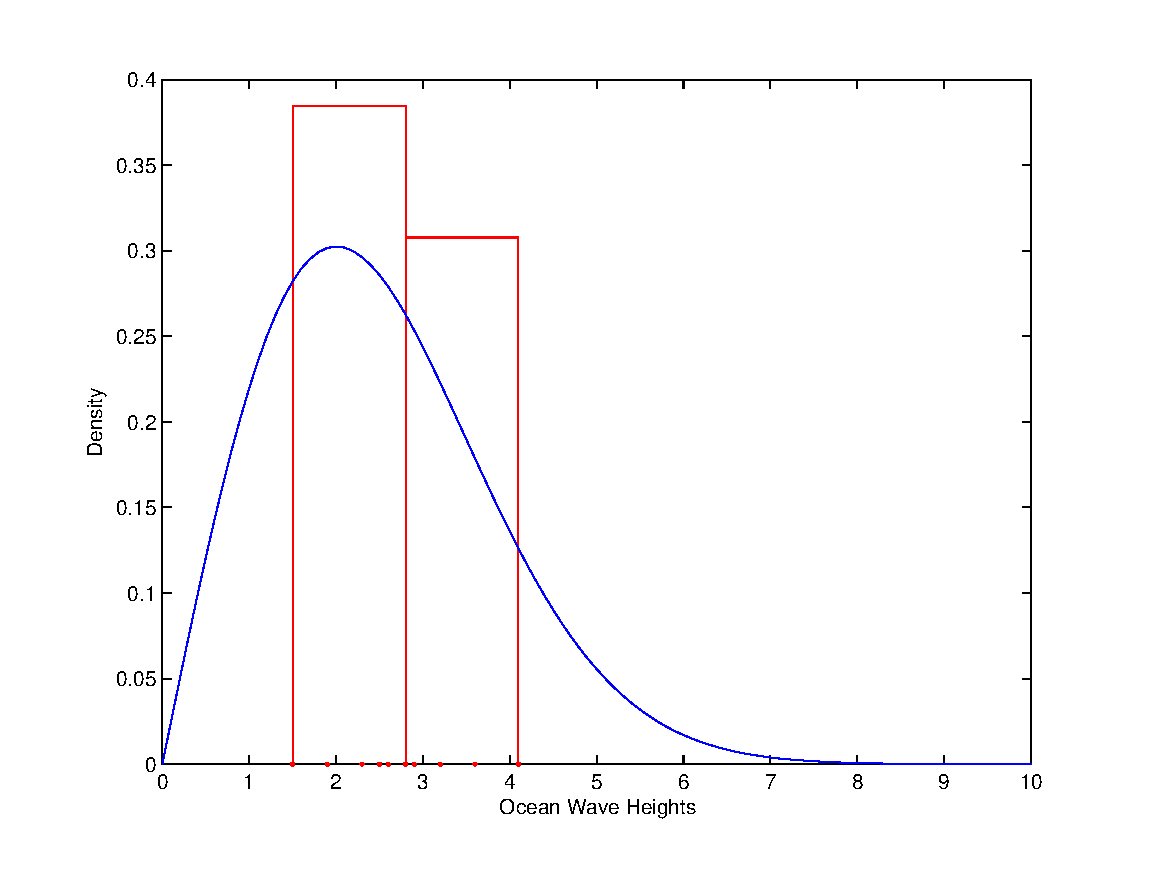
\includegraphics[width=6.5in]{figures/RayleighOceanHeightsMLE}}
\end{figure}
\begin{labwork}[6.7, p.~275 of Ang \& Tang]\label{LW:RayleighOceanHeightsMLE}
The distribution of ocean wave heights, $H$, may be modeled with the ${\rm Rayleigh}(\alpha)$ RV with parameter $\alpha$ and probability density function,
\[
f(h;\alpha) = \frac{h}{\alpha^2} \exp \left({-\frac{1}{2} (h/\alpha)^2}\right), \qquad h \in \Hz := [0,\infty) \ .
\]
The parameter space for $alpha$ is $\BB{A} = (0,\infty)$.  Suppose that the following measurements $h_1,h_2,\ldots,h_{10}$ of wave heights in meters were observed to be
\[
1.50, \  2.80, \ 2.50, \ 3.20, \ 1.90, \ 4.10, \ 3.60, \ 2.60, \ 2.90, \ 2.30 \ ,
\]
respectively.  Under the assumption that the $10$ samples are IID realisations from a ${\rm Rayleigh}(\alpha^*)$ RV with a fixed and unknown parameter $\alpha^*$, find the ML estimate $\widehat{\alpha}_{10}$ of $\alpha^*$.

We first obtain the log-likelihood function of $\alpha$ for the data $h_1,h_2,\ldots,h_n \overset{IID}{\sim} {\rm Rayleigh}(\alpha)$.
\begin{flalign*}
\ell(\alpha) & := \log(L(h_1,h_2,\ldots,h_n;\alpha)) = \log \left( \prod_{i=1}^n f(h_i;\alpha) \right) = \sum_{i=1}^n \log(f(h_i; \alpha))\\
& = \sum_{i=1}^n \log \left( \frac{h_i}{\alpha^2} e^{-\frac{1}{2} (h_i/\alpha)^2} \right) 
=  \sum_{i=1}^n \left( \log(h_i) - 2 \log(\alpha)  {-\frac{1}{2} (h_i/\alpha)^2} \right) \\
& = \sum_{i=1}^n \left( \log(h_i) \right) - 2 n \log(\alpha) - \sum_{i=1}^n \left(  \frac{1}{2} h_i^2 \alpha^{-2} \right) 
\end{flalign*}
Now, let us take the derivative with respect to $\alpha$,
\begin{flalign*}
\frac{\partial}{\partial \alpha} \left( \ell(\alpha) \right) 
& :=  \frac{\partial}{\partial \alpha} \left( \sum_{i=1}^n \left( \log(h_i) \right) - 2 n \log(\alpha) - \sum_{i=1}^n \left(  \frac{1}{2} h_i^2 \alpha^{-2} \right) \right) \\
& = \frac{\partial}{\partial \alpha} \left( \sum_{i=1}^n \left( \log(h_i) \right) \right) -  \frac{\partial}{\partial \alpha} \left( 2 n \log(\alpha) \right) -  \frac{\partial}{\partial \alpha} \left( \sum_{i=1}^n \left(  \frac{1}{2} h_i^2 \alpha^{-2} \right) \right) \\
& = 0 - 2n \frac{1}{\alpha} - \sum_{i=1}^n \left(  \frac{1}{2} h_i^2 (-2 \alpha^{-3}) \right)
= - 2n \alpha^{-1} + \alpha^{-3} \sum_{i=1}^n \left( h_i^2  \right)
\end{flalign*}
Next, we set the derivative to $0$, solve for $\alpha$, and set the solution equal to the ML estimate $\widehat{\alpha}_n$.
\begin{flalign*}
0 = \frac{\partial}{\partial \alpha} \left( \ell(\alpha) \right) 
& \iff 0 = - 2n \alpha^{-1} + \alpha^{-3} \sum_{i=1}^n h_i^2 \iff 2n \alpha^{-1} = \alpha^{-3} \sum_{i=1}^n h_i^2 \\
& \iff 2n \alpha^{-1} \alpha^{3} = \sum_{i=1}^n h_i^2 \iff \alpha^{2} = \frac{1}{2n} \sum_{i=1}^n h_i^2
\iff \widehat{\alpha}_n = \sqrt{  \frac{1}{2n} \sum_{i=1}^n h_i^2 }
\end{flalign*}
Therefore, the ML estimate of the unknown $\alpha^* \in \BB{A}$ on the basis of our $10$ observations $h_1,h_2,\ldots,h_{10}$ of wave heights is
\begin{flalign*}
\widehat{\alpha}_{10} & =  \sqrt{  \frac{1}{2*10} \sum_{i=1}^{10} h_i^2 } \\
& = \sqrt{ \frac{1}{20} \left( 1.50^2 + 2.80^2 + 2.50^2 + 3.20^2 + 1.90^2 + 4.10^2 + 3.60^2 + 2.60^2 + 2.90^2 + 2.30^2 \right)} \approxeq 2
\end{flalign*}
We use the following script file to compute the MLE $\widehat{\alpha}_{10}$ and plot the PDF at $\widehat{\alpha}_{10}$ in \hyperref[F:RayleighOceanHeightsMLE]{Figure~\ref*{F:RayleighOceanHeightsMLE}}.
\VrbMf[label=RayleighOceanHeightsMLE.m]{scripts/RayleighOceanHeightsMLE.m}
\begin{VrbM}
>> RayleighOceanHeightsMLE
AlphaHat =    2.0052
\end{VrbM}
\end{labwork}

%\begin{labwork}
%Choose some parameter $p\in[0,1]$ and some sample size $n$.  Then, using the {\sc Matlab} expression {\tt floor(rand(1,n)+p)} (See \hyperref[SIM:Bernoulli]{Simulation~\ref*{SIM:Bernoulli}}) simulate $n$ IID $\bernoulli(p)$ RVs $X_1,X_2,\ldots,X_n$.  Once you have generated the data, pretend that you don't know the $p$ used in your simulation and estimate $p$ using the sample mean estimator we have seen in \hyperref[EX:EstimatePFromNIIDBernoulliTrials]{Example~\ref*{EX:EstimatePFromNIIDBernoulliTrials}},  That is, compute the estimate $\widehat{p}_n=n^{-1}\sum_{i=1}^n x_i$ and also the approximate $95\%$ Normal-based confidence interval $C_n = \widehat{p}_n \pm 1.96 \sqrt{\frac{\widehat{p}_n(1-\widehat{p}_n)}{n}}$.

%For each value of $p \in [0, 1/100, 1/10, 2/10, 3/10, 4/10, 5/10, 6/10, 7/10, 8/10, 9/10, 9/100, 1]$,  generate $n$ IID $\bernoulli(p)$ samples where $n$ ranges in $\{10^i: i =1,2,3,4,5 \}$ and estimate $p$ from the simulated data of different sample sizes.  Do you intuitively agree with the behavior of the confidence intervals, in terms of the changes in their widths, as $n$ gets large for each of the fixed $p$'s ?  Is the point estimate $\widehat{p}_n$ approaching the $p$ from which the data were simulated for each of the fixed $p$'s as $n$ gets large ?
%For each value of $p$ as before, generate, say $1000$ data sets each of sample size $n \in \{10^i: i =1,2,3,4,5 \}$ and empirically study the coverage properties of the estimator.  That is, for each $p$ and $n$, find what fraction of the Normal-based  $95\%$ confidence intervals constructed from each of the $1000$ replicate data sets actually contain the parameter $p$ that they were simulated from.  Try to explain why coverage properties are both a function of how close $p$ is to the boundary of the the parameter space $[0,1]$ and the sample size $n$.  [Inspired by Russell Gribble]
%\end{labwork}

\section{Properties of the Maximum Likelihood Estimator}\label{S:PropsMLE}
Next, we list some nice properties of the ML Estimator $\widehat{\Theta}_n$ for the fixed and possibly unknown $\theta^* \in \BB{\Theta}$.
\begin{enumerate}
\item The ML Estimator is asymptotically consistent, i.e.~
$\widehat{\Theta}_n \overset{P}{\longrightarrow} \theta^*$.
\item The ML Estimator is asymptotically normal, i.e.~
$(\widehat{\Theta}_n - \theta^*) / \widehat{se}_n \rightsquigarrow \normal(0,1)$.
\item The estimated standard error of the ML Estimator, $\widehat{\mathsf{se}}_n$, can usually be computed analytically using the \hyperref[S:FisherInfo]{\bf Fisher Information}.
\item Because of the previous two properties, the $1-\alpha$ confidence interval can also be computed analytically as $\widehat{\Theta}_n \pm z_{\alpha/2} \widehat{\mathsf{se}}_n$.
\item The ML Estimator is {\bf equivariant}, i.e.~$\widehat{\psi}_n=g(\widehat{\theta}_n)$ is the ML Estimate of $\psi^*=g(\theta^*)$, for some smooth function $g(\theta)=\psi: \BB{\Theta} \to \BB{\Psi}$.  
\item We can also obtain the estimated standard error of the estimator 
$\widehat{\Psi}_n$ of $\psi^* \in \BB{\Psi}$ via the \hyperref[S:DeltaMethod]{\bf Delta Method}.
\item The ML Estimator is {\bf asymptotically optimal} or {\bf efficient}.  This means that the MLE has the smallest variance among the well-behaved class of estimators as the sample size gets larger.
\item ML Estimator is close to the Bayes estimator (obtained in the Bayesian inferential paradigm).
\end{enumerate}

\section{Fisher Information}\label{S:FisherInfo}
Let $X_1,X_2,\ldots,X_n \overset{IID}{\sim} f(X_1;\theta)$.  Here, $f(X_1;\theta)$ is the probability density function (pdf) or the probability mass function (pmf) of the RV $X_1$.  Since all RVs are identically distributed, we simply focus on $X_1$ without loss of generality.
\begin{definition}[Fisher Information]\label{D:FisherInfo}
The {\bf score function} of an RV $X$ for which the density is parameterised by $\theta$ is defined as:
\[
\mathscr{S}(X;\theta) := \frac{\partial log f(X;\theta)}{\partial \theta}, \qquad \text{and} \quad 
\E_{\theta} (\mathscr{S}(X;\theta))=0 \ .
\]
The {\bf Fisher Information} is
\begin{equation}\label{E:FisherInfo}
I_n := \V_{\theta} \left( \sum_{i=1}^n \mathscr{S}(X_i;\theta) \right) 
=  \sum_{i=1}^n \V_{\theta} \left( \mathscr{S}(X_i;\theta) \right) 
= n I_1(\theta),
\end{equation}
where $I_1$ is the Fisher Information of just one of the RVs $X_i$,e.g.~$X$:
\begin{eqnarray}
I_1 (\theta) &:=& \V_{\theta} \left( \mathscr{S}(X;\theta) \right) 
= \E_{\theta} \left(  \mathscr{S}^2(X,\theta) \right) \notag \\
&=& - \E_{\theta} \left(  \frac{\partial^2 log f(X;\theta)}{\partial^2 \theta} \right)
=
\begin{cases}
-\sum_{x \in \Xz}  \left( \frac{\partial^2 \log f(x;\theta)}{\partial^2 \theta} \right) f(x;\theta)  & \text{for discrete $X$}\\
-\int_{x \in \Xz}  \left( \frac{\partial^2 \log f(x;\theta)}{\partial^2 \theta} \right) f(x;\theta) dx  & \text{for continuous $X$} \qquad \label{E:FisherInfo1}
\end{cases}
\end{eqnarray}
\end{definition}
Next, we give a {\bf general method} for obtaining:
\begin{enumerate}
\item
The standard error $\mathsf{se}_n(\widehat{\Theta}_n)$ of {\bf any} maximum likelihood estimator $\widehat{\Theta}_n$ of the possibly unknown and fixed parameter of interest $\theta^* \in \BB{\Theta}$, and
\item The $1-\alpha$ confidence interval for $\theta^*$.
\end{enumerate}

\begin{prop}[Asymptotic Normality of the ML Estimator \& Confidence Intervals]
Let $\widehat{\Theta}_n$ be the maximum likelihood estimator of $\theta^* \in \BB{\Theta}$ with standard error $\mathsf{se}_n := \sqrt{\V_{\theta^*} (\widehat{\Theta}_n)}$.  Under appropriate regularity conditions, the following propositions are true:
\begin{enumerate}
\item The standard error $\mathsf{se}_n$ can be approximated by the side of a square whose area is the inverse Fisher Information at $\theta^*$, and the distribution of $\widehat{\Theta}_n$ approaches that of the $\normal(\theta^*, \mathsf{se}_n^2)$ distribution as the samples size $n$ gets larger.  In other terms:
\[
\mathsf{se}_n \approxeq \sqrt{1/I_n(\theta^*)} \qquad \text{and} \quad \frac{\widehat{\Theta}_n-\theta^*}{\mathsf{se}_n} \rightsquigarrow \normal(0,1)
\]
\item The approximation holds even if we substitute the ML Estimate $\widehat{\theta}_n$ for $\theta^*$ and use the estimated standard error $\widehat{\mathsf{se}}_n$ instead of $\mathsf{se}_n$.  Let $\widehat{\mathsf{se}}_n = \sqrt{1/I_n(\widehat{\theta}_n)}$.  Then:
\[
 \frac{\widehat{\Theta}_n-\theta^*}{\widehat{\mathsf{se}}_n} \rightsquigarrow \normal(0,1)
\]
\item Using the fact that $\widehat{\Theta}_n \rightsquigarrow \normal(\theta^*,\widehat{se}_n^2)$, we can construct the estimate of an approximate Normal-based $1-\alpha$ confidence interval as:
\[
C_n  =[\underline{C}_n, \overline{C}_n]= [\widehat{\theta}_n - z_{\alpha/2} \widehat{se}_n, \widehat{\theta}_n + z_{\alpha/2} \widehat{\mathsf{se}}_n]= \widehat{\theta}_n \pm z_{\alpha/2} \widehat{\mathsf{se}}_n
\]
\end{enumerate}
\end{prop}
Now, let us do an example.
\begin{example}[MLE and Confidence Interval for the IID $\poisson(\lambda)$ experiment]
Suppose the fixed parameter $\lambda^* \in \BB{\Lambda} = (0,\infty)$ is unknown.  Let $X_1,X_2,\ldots,X_n \overset{IID}{\sim} \poisson(\lambda^*)$.  We want to find the ML Estimate $\widehat{\lambda}_n$ of $\lambda^*$ and produce a $1-\alpha$ confidence interval for $\lambda^*$.

The MLE can be obtained as follows:

The likelihood function is:
\[
L(\lambda) := L(x_1,x_2,\ldots,x_n; \lambda) = \prod_{i=1}^n f(x_i;\lambda) = \prod_{i=1}^n e^{-\lambda} \frac{\lambda^x_i}{x_i!}
\]
Hence, the log-likelihood function is:
\begin{eqnarray}
\ell(\theta) := \log(L(\lambda)) 
&=&  \log \left( \prod_{i=1}^n e^{-\lambda} \frac{\lambda^{x_i}}{x_i!} \right) =  \sum_{i=1}^n \log \left(  e^{-\lambda} \frac{\lambda^{x_i}}{x_i!} \right) 
=  \sum_{i=1}^n \left( \log (e^{-\lambda}) + \log( \lambda^{x_i}) - \log({x_i!}) \right)  \notag \\
&=& \sum_{i=1}^n \left({-\lambda} + x_i \log( \lambda) - \log({x_i!}) \right) 
= \sum_{i=1}^n {-\lambda} + \sum_{i=1}^n x_i \log( \lambda) - \sum_{i=1}^n \log({x_i!})  \notag \\
&=& n ( {-\lambda}) + \log( \lambda) \left( \sum_{i=1}^n x_i \right) - \sum_{i=1}^n \log({x_i!})  \notag 
\end{eqnarray}
Next, take the derivative of $\ell(\lambda)$:
\[
\frac{\partial}{\partial \lambda} \ell (\lambda) 
= \frac{\partial}{\partial \lambda} \left(  n ( {-\lambda}) + \log( \lambda) \left( \sum_{i=1}^n x_i \right) - \sum_{i=1}^n \log({x_i!})  \right)
= n(-1) + \frac{1}{\lambda} \left( \sum_{i=1}^n x_i \right) + 0
\]
and set it equal to $0$ to solve for $\lambda$, as follows:
\[
0 = n(-1) + \frac{1}{\lambda} \left( \sum_{i=1}^n x_i \right) + 0 \iff n = \frac{1}{\lambda} \left( \sum_{i=1}^n x_i \right) \iff \lambda =  \frac{1}{n} \left( \sum_{i=1}^n x_i \right) = \overline{x}_n
\]
Finally, the ML Estimator of $\lambda^*$ is $\widehat{\Lambda}_n = \overline{X}_n$ and the ML estimate is $\widehat{\lambda}_n = \overline{x}_n$.

Now, we want an $1-\alpha$ confidence interval for $\lambda^*$ using the $\widehat{\mathsf{se}}_n \approxeq \sqrt{1/I_n(\widehat{\lambda}_n)}$ that is based on the Fisher Information $I_n(\lambda) = n I_1(\lambda)$ given in \eqref{E:FisherInfo}.  We need $I_1$ given in \eqref{E:FisherInfo1}.  Since $X_1,X_2,\ldots,X_n \sim \poisson(\lambda)$, we have discrete RVs:
\[
I_1 = -\sum_{x \in \Xz}  \left( \frac{\partial^2 \log (f(x;\lambda))}{\partial^2 \lambda} \right) f(x;\lambda) = -\sum_{x =0}^{\infty}  \left( \frac{\partial^2 \log (f(x;\lambda))}{\partial^2 \lambda} \right) f(x;\lambda)
\]
First find 
\begin{eqnarray}
\frac{\partial^2 \log (f(x;\lambda))}{\partial^2 \lambda}
&=& \frac{\partial}{\partial \lambda} \left( \frac{\partial} {\partial \lambda} \log \left(  f(x;\lambda) \right
) \right)
=  \frac{\partial}{\partial \lambda} \left( \frac{\partial} {\partial \lambda} \log \left( e^{-\lambda} \frac{\lambda^x}{x!} \right) \right) \notag \\
&=& \frac{\partial}{\partial \lambda} \left( \frac{\partial} {\partial \lambda} \left( -\lambda + x \log(\lambda)-\log({x!}) \right) \right)
= \frac{\partial}{\partial \lambda} \left( -1 + \frac{x}{\lambda}-0 \right)
= -\frac{x}{\lambda^2} \notag
\end{eqnarray}
\end{example}
Now, substitute the above expression into the right-hand side of $I_1$ to obtain:
\[
I_1= - \sum_{x=0}^{\infty} \left( -\frac{x}{\lambda^2} \right) f(x;\lambda)
= \frac{1}{\lambda^2} \sum_{x=0}^{\infty} \left( x \right) f(x;\lambda)
= \frac{1}{\lambda^2} \sum_{x=0}^{\infty} \left( x \right) e^{-\lambda} \frac{\lambda^x}{x!} 
=  \frac{1}{\lambda^2} \E_{\lambda}(X)
= \frac{1}{\lambda^2} \lambda
=\frac{1}{\lambda}
\]
In the third-to-last step above, we recognise the sum as the expectation of the $\poisson(\lambda)$ RV $X$, namely $\E_{\lambda}(X)=\lambda$.  Therefore, the estimated standard error is:
\[
\widehat{\mathsf{se}}_n \approxeq \sqrt{1/I_n(\widehat{\lambda}_n)}
= \sqrt{1/(n I_1(\widehat{\lambda}_n))}
= \sqrt{1/(n (1/\widehat{\lambda}_n))}
= \sqrt{\widehat{\lambda}_n/n}
\]
and the approximate $1-\alpha$ confidence interval is
\[
\widehat{\lambda}_n \pm z_{\alpha/2} \widehat{\mathsf{se}}_n 
= \widehat{\lambda}_n \pm z_{\alpha/2} \sqrt{\widehat{\lambda}_n/n}
\]

Thus, using the MLE and the estimated standard error via the Fisher Information, we can carry out point estimation and confidence interval construction in {\bf most} parametric families of RVs encountered in typical engineering applications.  

\begin{example}[Fisher Information of the $\bernoulli$ Experiment]\label{EX:BernoulliFisherInfo}
Suppose $X_1,X_2,\ldots,X_n \overset{IID}{\sim}$ $\bernoulli(\theta^*)$.  Also, suppose that $\theta^* \in \BB{\Theta} = [0,1]$ is unknown.  We have already shown in \hyperref[EX:CoinTossingML]{Example~\ref*{EX:CoinTossingML}} that the ML estimator of $\theta^*$ is $\widehat{\theta}_n = \overline{X}_n$.  Using the identity:
\[
\widehat{\mathsf{se}}_n = \frac{1}{\sqrt{I_n(\widehat{\theta}_n)}}
\]
(1) we can compute $\widehat{\mathsf{se}}_n(\widehat{\Theta}_n)$, the estimated standard error  of the unknown parameter $\theta^*$ as follows:
\begin{flalign*}
\widehat{\mathsf{se}}_n (\widehat{\Theta}_n) &= \frac{1}{\sqrt{I_n(\widehat{\theta}_n)}} =   \frac{1}{\sqrt{n I_1(\widehat{\theta}_n)}} \ .
\end{flalign*}
So, we need to first compute $I_1(\theta)$, the Fisher Information of one sample.  Due to \eqref{E:FisherInfo1} and the fact that the $\bernoulli(\theta^*)$ distributed RV $X$ is discrete with probability mass function $f(x;\theta)=\theta^{x} (1-\theta)^{1-x}$, for $x\in \Xz := \{0,1\}$, we have,
\begin{flalign*}
I_1(\theta) &= - \E_{\theta} \left(  \frac{\partial^2 log f(X;\theta)}{\partial^2 \theta} \right) = - \sum_{x \in \Xz = \{0,1\}} \left( \frac{\partial^2 \log \left( \theta^{x} (1-\theta)^{1-x} \right)}{\partial^2 \theta} \right) \theta^{x} (1-\theta)^{1-x} \\
\end{flalign*}
Next, let us compute,
\begin{flalign*}
\frac{\partial^2 \log \left( \theta^{x} (1-\theta)^{1-x} \right)}{\partial^2 \theta} & :=
\frac{\partial}{\partial \theta} \left( \frac{\partial}{\partial \theta} \left( \log \left( \theta^{x} (1-\theta)^{1-x} \right) \right) \right) = 
\frac{\partial}{\partial \theta} \left( \frac{\partial}{\partial \theta} \left( x \log(\theta) + (1-x) \log(1-\theta)  \right) \right) \\
& = \frac{\partial}{\partial \theta} \left(  x \theta^{-1} + (1-x)(1-\theta)^{-1} (-1)  \right) 
=\frac{\partial}{\partial \theta} \left(  x \theta^{-1} - (1-x)(1-\theta)^{-1}  \right)  \\
&=  x (-1) \theta^{-1-1} - (1-x) (-1) (1-\theta)^{-1-1} (-1)
= - x \theta^{-2} - (1-x) (1-\theta)^{-2}
\end{flalign*}
Now, we compute the expectation $I_1$, i.e.~the sum over the two possible values of $x\in\{0,1\}$,
\begin{flalign*}
I_1(\theta) &= - \sum_{x \in \Xz = \{0,1\}} \left( \frac{\partial^2 \log \left( \theta^{x} (1-\theta)^{1-x} \right)}{\partial^2 \theta} \right) \theta^{x} (1-\theta)^{1-x} \\
& = - \left( \left(- 0 \ \theta^{-2} - (1-0) (1-\theta)^{-2} \right) \theta^{0} (1-\theta)^{1-0} + \left( - 1 \ \theta^{-2} - (1-1) (1-\theta)^{-2} \right) \theta^{1} (1-\theta)^{1-1} \right) \\
& = - \left( \left(0 - 1 (1-\theta)^{-2} \right) \ 1 \ (1-\theta)^1 + \left( - \theta^{-2} - 0  \right) \theta^1 \ 1 \right) 
=  (1-\theta)^{-2} (1-\theta)^1 +  \theta^{-2} \theta^1 \\
& = (1-\theta)^{-1} +  \theta^{-1}  = \frac{1}{1-\theta} + \frac{1}{\theta} 
= \frac{\theta}{\theta (1-\theta)} +  \frac{1-\theta}{\theta (1-\theta)} 
= \frac{\theta+(1 - \theta)}{\theta (1-\theta)} = \frac{1}{\theta (1-\theta)}
\end{flalign*}
Therefore, the desired estimated standard error of our estimator, can be obtained by substituting the ML estimate $\widehat{\theta}_n=\overline{x}_n := n^{-1}\sum_{i=1}^n x_i$ of the unknown $\theta^*$ as follows:
\begin{flalign*}
\widehat{\mathsf{se}}_n(\widehat{\theta}_n) = \frac{1}{\sqrt{I_n(\widehat{\theta}_n)}} 
 = \frac{1}{\sqrt{n I_1(\widehat{\theta}_n)}}
 = \sqrt{\frac{1}{n \frac{1}{\widehat{\theta}_n (1-\widehat{\theta}_n)} }} 
= \sqrt{\frac{\widehat{\theta}_n(1-\widehat{\theta}_n)}{n}} 
= \sqrt{\frac{\overline{x}_n(1-\overline{x}_n)}{n}}  \ .
\end{flalign*}
(2) Using $\widehat{\mathsf{se}}_n(\widehat{\theta}_n)$ we can construct an approximate $95\%$ confidence interval $C_n$ for $\theta^*$, due to the asymptotic normality of the ML estimator of $\theta^*$, as follows:
\[
C_n = \widehat{\theta}_n \pm 1.96 \sqrt{\frac{\widehat{\theta}_n(1-\widehat{\theta}_n)}{n}}
= \overline{x}_n \pm 1.96 \sqrt{\frac{\overline{x}_n(1-\overline{x}_n)}{n}}
\]
Recall that $C_n$ is the realisation of a random set based on your observed samples or data  $x_1,x_2,\ldots,x_n$.   Furthermore, $C_n$'s construction procedure ensures the engulfing of the unknown $\theta^*$ with probability approaching $0.95$ as the sample size $n$ gets large.

%(3) Flip any New Zealand coin as identically and independently as possible exactly $30$ times and record the outcomes ($1$ for heads and $0$ for tails).  Report the ML point estimate and the $95\%$ confidence interval from your data.  Do you think that the way you have flipped your coin and the outcomes you have witnessed can hint at the fairness ($\theta^*=0.5$) or unfairness ($\theta^*\neq0.5$) of the coin.  Write a couple of sentences to make your case.    [Take the time to flip coins this many times in a row, if you have not done so already.  Be honest and really do it.  I flipped an American quarter $100$ times to produce the data in \hyperref[EX:EstimatePFromNIIDBernoulliTrials]{Example \ref*{EX:EstimatePFromNIIDBernoulliTrials}}].
\end{example}

\begin{example}[[Fisher Information of the $\exponential$ Experiment]]\label{EX:ExponentialFisherInfo}
Let us get our hands dirty with a continuous RV next.  Let $X_1,X_2,\ldots,X_n \overset{IID}{\sim} \exponential(\lambda^*)$.  We saw that the ML estimator of $\lambda^* \in \BB{\Lambda}=(0,\infty)$ is $\widehat{\Lambda}_n = 1/\overline{X}_n$ and its ML estimate is $\widehat{\lambda}_n=1/\overline{x}_n$, where $x_1,x_2,\ldots,x_n$ are our observed data.

(1) Let us obtain the Fisher Information $I_n$ for this experiment to find the standard error:
\[
\widehat{\mathsf{se}}_n(\widehat{\Lambda}_n) = \frac{1}{\sqrt{I_n(\widehat{\lambda}_n)}}
= \frac{1}{\sqrt{n I_1(\widehat{\lambda}_n)}}
\]
and construct an approximate $95\%$ confidence interval for $\lambda^*$ using the asymptotic normality of its ML estimator $\widehat{\Lambda}_n$.  

So, we need to first compute $I_1(\theta)$, the Fisher Information of one sample.  Due to \eqref{E:FisherInfo1} and the fact that the $\exponential(\lambda^*)$ distributed RV $X$ is continuous with probability density function $f(x;\lambda)=\lambda e^{-\lambda x}$, for $x\in \Xz := [0,\infty)$, we have,
\begin{flalign*}
I_1(\theta) &= - \E_{\theta} \left(  \frac{\partial^2 log f(X;\theta)}{\partial^2 \theta} \right) = - \int_{x \in \Xz = [0,\infty)} \left( \frac{\partial^2 \log \left( \lambda e^{-\lambda x} \right)}{\partial^2 \lambda} \right) \lambda e^{-\lambda x} \ dx
\end{flalign*}
Let us compute the above integrand next.
\begin{flalign*}
\frac{\partial^2 \log \left( \lambda e^{-\lambda x} \right)}{\partial^2 \lambda}
&:= 
\frac{\partial}{\partial \lambda} \left( \frac{\partial}{\partial \lambda} \left( \log \left( \lambda e^{-\lambda x} \right)   \right) \right)
= \frac{\partial}{\partial \lambda} \left( \frac{\partial}{\partial \lambda} \left( \log(\lambda) + \log(e^{-\lambda x} \right) \right) \\
&= \frac{\partial}{\partial \lambda} \left( \frac{\partial}{\partial \lambda} \left( \log(\lambda) -\lambda x \right) \right) 
= \frac{\partial}{\partial \lambda} \left( {\lambda}^{-1} - x \right) = - \lambda^{-2} - 0 = -\frac{1}{\lambda^2}
\end{flalign*}
Now, let us evaluate the integral by recalling that the expectation of the constant $1$ is 1 for any RV $X$ governed by some parameter, say $\theta$.  For instance when $X$ is a continuous RV, $\E_{\theta}(1) = \int_{x \in \Xz} 1 \ f(x;\theta) =  \int_{x \in \Xz} \ f(x;\theta) = 1$.  Therefore, the Fisher Information of one sample is
\begin{flalign*}
I_1(\theta) = - \int_{x \in \Xz = [0,\infty)} \left( \frac{\partial^2 \log \left( \lambda e^{-\lambda x} \right)}{\partial^2 \lambda} \right) \lambda e^{-\lambda x} \ dx
 &=  - \int_{0}^{\infty} \left(-\frac{1}{\lambda^2} \right) \lambda e^{-\lambda x} \ dx \\
& = -  \left(-\frac{1}{\lambda^2} \right) \int_{0}^{\infty} \lambda e^{-\lambda x} \ dx = \frac{1}{\lambda^2} \ 1 = \frac{1}{\lambda^2}
\end{flalign*}
Now, we can compute the desired estimated standard error, by substituting in the ML estimate $\widehat{\lambda}_n = 1/(\overline{x}_n) := 1 / \left( \sum_{i=1}^n x_i \right)$ of $\lambda^*$, as follows:
\[
\widehat{\mathsf{se}}_n(\widehat{\Lambda}_n) = \frac{1}{\sqrt{I_n(\widehat{\lambda}_n)}}
= \frac{1}{\sqrt{n I_1(\widehat{\lambda}_n)}} 
= \frac{1}{\sqrt{n \frac{1}{\widehat{\lambda}_n^2} }}
= \frac{\widehat{\lambda}_n}{\sqrt{n}}
= \frac{1}{\sqrt{n} \ \overline{x}_n}
\]
Using $\widehat{\mathsf{se}}_n(\widehat{\lambda}_n)$ we can construct an approximate $95\%$ confidence interval $C_n$ for $\lambda^*$, due to the asymptotic normality of the ML estimator of $\lambda^*$, as follows:
\[
C_n 
= \widehat{\lambda}_n \pm 1.96 \frac{\widehat{\lambda}_n}{\sqrt{n}}
= \frac{1}{\overline{x}_n} \pm 1.96 \frac{1}{\sqrt{n} \ \overline{x}_n} \enspace .
\]
Let us compute the ML estimate and the $95\%$ confidence interval for the rate parameter for the waiting times at the Orbiter bus-stop (see \hyperref[LW:ExponentialMLEOrbiter]{labwork~\ref*{LW:ExponentialMLEOrbiter}}).  The sample mean $\overline{x}_{132}=9.0758$ and the ML estimate is:
$$\widehat{\lambda}_{132}=1/\overline{x}_{132}=1/9.0758=0.1102 \enspace ,$$
and the $95\%$ confidence interval is:  
\[
C_n 
= \widehat{\lambda}_{132} \pm 1.96 \frac{\widehat{\lambda}_{132}}{\sqrt{132}}
= \frac{1}{\overline{x}_{132}} \pm 1.96 \frac{1}{\sqrt{132} \ \overline{x}_{132}} = 0.1102 \pm 1.96 \cdot 0.0096 = [0.0914, 0.1290] \enspace .
\]
Notice how poorly the exponential PDF $f(x;\widehat{\lambda}_{132}=0.1102)$ and the DF $F(x;\widehat{\lambda}_{132}=0.1102)$ based on the MLE fits with the histogram and the empirical DF, respectively, in \hyperref[F:ExponentialMLECIOrbiter]{Figure~\ref*{F:ExponentialMLECIOrbiter}}, despite  taking the the confidence interval into account.  This is a further indication of the inadequacy of our parametric model.
\end{example}

\begin{figure}[htpb]
\caption{Plot of $\log(L(\lambda))$ as a function of the parameter $\lambda$, the MLE 
$\widehat{\lambda}_{132}=0.1102$ and $95\%$ confidence interval $C_n=[0.0914, 0.1290]$ for Fenemore-Wang Orbiter Waiting Times Experiment from STAT 218 S2 2007.  The PDF and the DF at (1) the MLE $0.1102$ (black), (2) lower $95\%$ confidence bound $0.0914$ (red) and (3) upper $95\%$ confidence bound $0.1290$ (blue) are compared with a histogram and the empirical DF.
\label{F:ExponentialMLECIOrbiter}}
\centering   \makebox{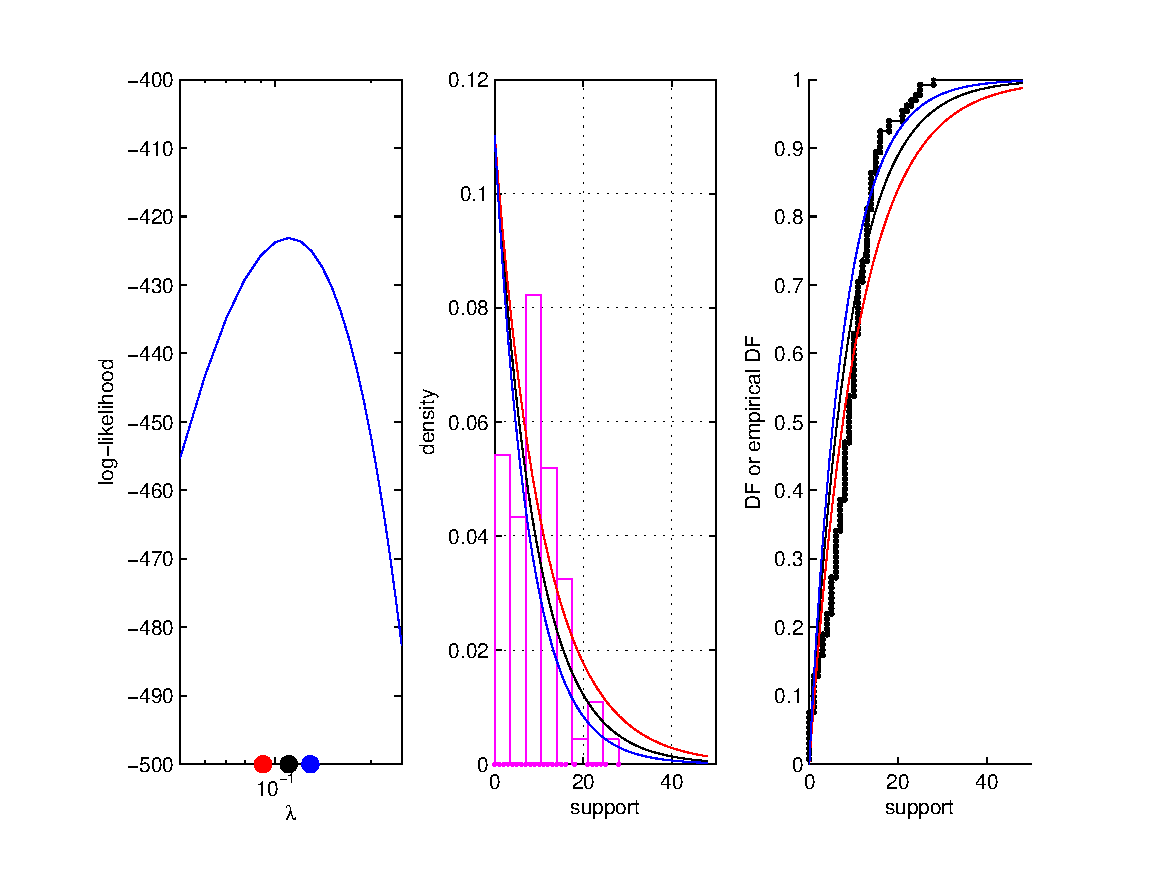
\includegraphics[width=6.5in]{figures/ExponentialMLECIOrbiter}}
\end{figure}

\begin{labwork}[Maximum likelihood estimation for Orbiter bus-stop]\label{LW:ExponentialMLECIOrbiter}
The above analysis was undertaken with the following M-file:
\VrbMf[label=ExponentialMLECIOrbiter.m]{scripts/ExponentialMLECIOrbiter.m}
A call to the script generates \hyperref[F:ExponentialMLECIOrbiter]{Figure~\ref*{F:ExponentialMLECIOrbiter}} and the following output of the sample mean, MLE, sample size, standard error and the $95\%$ confidence interval.  
\begin{VrbM}
>> ExponentialMLECIOrbiter
SampleMean =    9.0758
MLE =    0.1102
n =   132
StdErr =    0.0096
MLE95CI =    0.0914    0.1290
\end{VrbM}
\end{labwork}

\begin{labwork} [Maximum likelihood estimation for your bus-stop]\label{LW:IDSeededBusStopMLECI}
Recall \hyperref[LW:Next7Buses]{labwork~\ref*{LW:Next7Buses}} where you modeled the arrival of buses using $\exponential(\lambda^*=0.1)$ distributed inter-arrival time with a mean of $1/\lambda^*=10$ minutes.  Using the data of these seven inter-arrival times at your ID-seeded bus stop and pretending that you do not know the true $\lambda^*$, report (1) the ML estimate of $\lambda^*$, (2) $95\%$ confidence interval for it and (3) whether the true value $\lambda^*=1/10$ is engulfed by your confidence interval.  
\end{labwork}

\section{Delta Method}\label{S:DeltaMethod}
A more general estimation problem of interest concerns some function of the parameter $\theta \in \BB{\Theta}$, say $g(\theta)=\psi:\BB{\Theta} \to \BB{\Psi}$.  So, $g(\theta)=\psi$ is a function from the parameter space $\BB{\Theta}$ to $\BB{\Psi}$.  Thus, we are not only interested in estimating the fixed and possibly unknown $\theta^* \in \BB{\Theta}$ using the ML estimator $\widehat{\Theta}_n$ and its ML estimate $\widehat{\theta}_n$, but also in estimating $\psi^* = g(\theta^*) \in \BB{\Psi}$ via an estimator $\widehat{\Psi}_n$ and its estimate $\widehat{\psi}_n$.  We exploit the equivariance property of the ML estimator $\widehat{\Theta}_n$ of $\theta^*$ and use the Delta method to find the following analytically:
\begin{enumerate}
\item The ML estimator of $\psi^*=g(\theta^*) \in \BB{\Psi}$ is 
$$\boxed{\widehat{\Psi}_n = g(\widehat{\Theta}_n)}$$ 
and its point estimate is 
$$\boxed{\widehat{\psi}_n=g(\widehat{\theta}_n)}$$
\item Suppose $g(\theta)=\psi:\BB{\Theta} \to \BB{\Psi}$ is {\bf any} smooth function of $\theta$, i.e.~$g$ is differentiable, and $g'(\theta) := \frac{\partial}{\partial \theta}g(\theta) \neq 0$.  Then, the distribution of the ML estimator $\widehat{\Psi}_n$ is asymptotically $\normal(\psi^*, {\widehat{\mathsf{se}}_n(\widehat{\Psi}_n)}^2)$, i.e.:
\[
\boxed{
\frac{\widehat{\Psi}_n - \psi^*}{\widehat{\mathsf{se}}_n(\widehat{\Psi}_n)} \rightsquigarrow
\normal(0,1)
}
\]
where the standard error $\widehat{\mathsf{se}}_n(\widehat{\Psi}_n)$ of the ML estimator $\widehat{\Psi}_n$ of the unknown quantity $\psi^* \in \BB{\Psi}$ can be obtained from the standard error $\widehat{\mathsf{se}}_n(\widehat{\Theta}_n)$ of the ML estimator $\widehat{\Theta}_n$ of the parameter $\theta^* \in \BB{\Theta}$, as follows:
\[
\boxed{
\widehat{\mathsf{se}}_n(\widehat{\Psi}_n) = |g'(\widehat{\theta}_n)| \widehat{\mathsf{se}}_n(\widehat{\Theta}_n)
}
\]
\item Using $\normal(\psi^*, {\widehat{\mathsf{se}}_n(\widehat{\Psi}_n)}^2)$, we can construct the estimate of an approximate Normal-based $1-\alpha$ confidence interval for $\psi^* \in \BB{\Psi}$:
\[
\boxed{
C_n  =[\underline{C}_n, \overline{C}_n]= \widehat{\psi}_n \pm z_{\alpha/2} {\widehat{\mathsf{se}}_n(\widehat{\psi}_n)}
}
\]
\end{enumerate}

Let us do an example next.
\begin{example}
Let $X_1,X_2,\ldots,X_n \overset{IID}{\sim} \bernoulli(\theta^*)$.  Let $\psi=g(\theta)=\log(\theta/(1-\theta))$.  Suppose we are interested in producing a point estimate and confidence interval for $\psi^*=g(\theta^*)$.  We can use the Delta method as follows: 

First, the estimated standard error of the ML estimator of $\theta^*$, as shown in \hyperref[EX:BernoulliFisherInfo]{Example~\ref*{EX:BernoulliFisherInfo}}, is
\[
\widehat{\mathsf{se}}_n(\widehat{\Theta}_n) = \sqrt{\frac{\widehat{\theta}_n (1-\widehat{\theta}_n)}{n}} \ .
\]
The ML estimator of $\psi^*$ is:
$$\widehat{\Psi}_n=\log(\widehat{\Theta}_n / (1-\widehat{\Theta}_n))$$ 
and the ML estimate of $\psi^*$ is:
$$\widehat{\psi}_n=\log(\widehat{\theta}_n / (1-\widehat{\theta}_n)) \ .$$
Since, $g'(\theta) = 1/(\theta (1-\theta))$, by the Delta method, the estimated standard error of the ML estimator of $\psi^*$ is:
\[
\widehat{\mathsf{se}}_n(\widehat{\Psi}_n) = |g'(\widehat{\theta}_n)| (\widehat{\mathsf{se}}_n(\widehat{\Theta}_n))
= \frac{1}{\widehat{\theta}_n (1-\widehat{\theta}_n)} \sqrt{\frac{\widehat{\theta}_n (1-\widehat{\theta}_n)}{n}}
= \frac{1}{\sqrt{n\widehat{\theta}_n (1-\widehat{\theta}_n)}}
= \frac{1}{\sqrt{n \overline{x}_n (1-\overline{x}_n)}} \ .
\]
An approximate $95\%$ confidence interval for $\psi^*=\log(\theta^*/(1-\theta^*))$ is:
\[
\widehat{\psi}_n \pm \frac{1.96}{\sqrt{n \widehat{\theta}_n (1-\widehat{\theta}_n)}}
= \log(\widehat{\theta}_n / (1-\widehat{\theta}_n)) \pm \frac{1.96}{\sqrt{n \widehat{\theta}_n (1-\widehat{\theta}_n)}}
= \log(\overline{x}_n / (1-\overline{x}_n)) \pm \frac{1.96}{\sqrt{n \overline{x}_n (1-\overline{x}_n)}} \ .
\]
\end{example}

\begin{example}[Delta Method for a $\normal$ Experiment]\label{EX:NormalDelta}
Let us try the Delta method on a continuous RV.  Let $X_1,X_2,\ldots,X_n \overset{IID}{\sim} \normal(\mu^*, {\sigma^*}^2)$.  Suppose that $\mu^*$ is known and $\sigma^*$ is unknown.  Let us derive the ML estimate $\widehat{\psi}_n$ of $\psi^* = \log(\sigma^*)$ and a $95\%$ confidence interval for it in 6 steps.

(1) First let us find the log-likelihood function $\ell(\sigma)$ 
\begin{flalign*}
\ell(\sigma) 
& := \log (L(\sigma)) := \log( L(x_1,x_2,\ldots,x_n; \sigma)) = \log \left( \prod_{i=1}^n f(x_i; \sigma) \right) = \sum_{i=1}^n \log \left( f(x_i; \sigma) \right) \\
& = \sum_{i=1}^n \log \left( \frac{1}{\sigma \sqrt{2 \pi}}
 \exp{\left( - \frac{1}{2 \sigma^2} (x_i-\mu)^2 \right)} \right) \quad \because \text{\scriptsize{$f(x_i;\sigma)$ in \eqref{E:Normalpdf} is pdf of $\normal(\mu,\sigma^2)$ RV with known $\mu$}} \\
 & =  \sum_{i=1}^n \left( \log \left( \frac{1}{\sigma \sqrt{2 \pi}} \right) +
 \log \left( \exp{\left( - \frac{1}{2 \sigma^2} (x_i-\mu)^2 \right)} \right) \right) \\
& =  \sum_{i=1}^n \log \left( \frac{1}{\sigma \sqrt{2 \pi}} \right) +
 \sum_{i=1}^n \left( - \frac{1}{2 \sigma^2} (x_i-\mu)^2 \right)
 = n \log \left( \frac{1}{\sigma \sqrt{2 \pi}} \right) +
\left( - \frac{1}{2 \sigma^2} \right) \sum_{i=1}^n (x_i-\mu)^2 \\
& = n \left( \log \left( \frac{1}{\sqrt{2 \pi}} \right) + \log \left( \frac{1}{\sigma} \right) \right) -
\left( \frac{1}{2 \sigma^2} \right) \sum_{i=1}^n (x_i-\mu)^2 \\
& = n \log \left({\sqrt{2 \pi}}^{-1} \right) + n \log \left( \sigma^{-1} \right)  -
\left( \frac{1}{2 \sigma^2} \right) \sum_{i=1}^n (x_i-\mu)^2 \\
& = - n \log \left({\sqrt{2 \pi}} \right) - n \log \left( \sigma \right)  -
\left( \frac{1}{2 \sigma^2} \right) \sum_{i=1}^n (x_i-\mu)^2 
\end{flalign*}
(2) Let us find its derivative with respect to the unknown parameter $\sigma$ next.
\begin{flalign*}
\frac{\partial}{\partial \sigma } \ell(\sigma) 
& :=
\frac{\partial}{\partial \sigma } \left( - n \log \left({\sqrt{2 \pi}} \right) - n \log \left( \sigma \right)  -
\left( \frac{1}{2 \sigma^2} \right) \sum_{i=1}^n (x_i-\mu)^2 \right) \\
& = \frac{\partial}{\partial \sigma } \left( - n \log \left({\sqrt{2 \pi}} \right) \right) 
-  \frac{\partial}{\partial \sigma } \left( n \log \left( \sigma \right) \right) 
-  \frac{\partial}{\partial \sigma } \left( \left( \frac{1}{2 \sigma^2} \right) \sum_{i=1}^n (x_i-\mu)^2 \right)  \\
& = 0 - n  \frac{\partial}{\partial \sigma } \left( \log(\sigma) \right) - \left( \frac{1}{2} \sum_{i=1}^n (x_i-\mu)^2 \right) \frac{\partial}{\partial \sigma } \left( \sigma^{-2} \right) \\
& = -n \sigma^{-1} - \left( \frac{1}{2} \sum_{i=1}^n (x_i-\mu)^2 \right) \left(-2  \sigma^{-3} \right)
 = -n \sigma^{-1} +  \sigma^{-3} \sum_{i=1}^n (x_i-\mu)^2
\end{flalign*}
(3) Now, let us set the derivative equal to $0$ and solve for $\sigma$.
\begin{flalign*}
0  =  -n \sigma^{-1} +  \sigma^{-3} \sum_{i=1}^n (x_i-\mu)^2 
& \iff n \sigma^{-1}   =   \sigma^{-3} \sum_{i=1}^n (x_i-\mu)^2 
 \iff n \sigma^{-1} \sigma^{+3}    =   \sum_{i=1}^n (x_i-\mu)^2 \\
& \iff n \sigma^{-1+3}    =   \sum_{i=1}^n (x_i-\mu)^2 
\iff n \sigma^{2}    =   \sum_{i=1}^n (x_i-\mu)^2 \\
& \iff \sigma^{2}    =  \left( \sum_{i=1}^n (x_i-\mu)^2 \right) / n
\iff \sigma = \sqrt{\sum_{i=1}^n(x_i-\mu)^2/n}
\end{flalign*}
Finally, we set the solution, i.e.~the maximiser of the concave-down log-likelihood function of $\sigma$ with a known and fixed $\mu^*$ as our ML estimate $\widehat{\sigma}_n=\sqrt{\sum_{i=1}^n(x_i-\mu^*)^2/n}$.  Analogously, the ML estimator of $\sigma^*$ is $\widehat{\Sigma}_n=\sqrt{\sum_{i=1}^n(X_i-\mu^*)^2/n}$.  Don't confuse $\Sigma$, the upper-case sigma, with $\sum_{i=1}^n \bigcirc_i $, the summation over some $\bigcirc_i$'s.  This is usually clear from the context.

(4) Next, let us get the estimated standard error $\widehat{se}_n$ for the estimator of $\sigma^*$ via Fisher Information.  The Log-likelihood function of $\sigma$, based on one sample from the $\normal(\mu, \sigma^2)$ RV with known $\mu$ is,
\[
\log f(x;\sigma) = \log \left( \frac{1}{\sigma \sqrt{2 \pi}}
 \exp{\left( - \frac{1}{2 \sigma^2} (x-\mu)^2 \right)} \right)
 = - \log \left({\sqrt{2 \pi}} \right) - \log \left( \sigma \right)  -
\left( \frac{1}{2 \sigma^2} \right)  (x-\mu)^2 \\
\]
Therefore, in much the same way as in part (2) earlier,
\begin{flalign*}
\frac{\partial^2 \log f(x;\sigma)}{\partial^2 \sigma} 
& := \frac{\partial}{\partial \sigma} 
\left( 
\frac{\partial}{\partial \sigma} 
\left(  
- \log \left({\sqrt{2 \pi}} \right) - \log \left( \sigma \right)  - \left( \frac{1}{2 \sigma^2} \right)  
(x-\mu)^2 \right) \right) \\
& = \frac{\partial}{\partial \sigma} 
\left( -\sigma^{-1}  +  \sigma^{-3} 
(x-\mu)^2 \right) 
 = \sigma^{-2}  -3  \sigma^{-4} (x-\mu)^2 
\end{flalign*}
Now, we compute the Fisher Information of one sample as an expectation of the continuous RV $X$ over $\Xz = (-\infty,\infty)$ with density $f(x;\sigma)$,
\begin{flalign*}
I_1(\sigma) 
& = - \int_{x \in \Xz = (-\infty,\infty)} \left( \frac{\partial^2 \log f(x;\sigma)}{\partial^2 \lambda} \right) f(x;\sigma) \ dx
 =  - \int_{-\infty}^{\infty} \left( \sigma^{-2}  -3  \sigma^{-4} (x-\mu)^2  \right) f(x;\sigma) \ dx \\
 &=   \int_{-\infty}^{\infty} -\sigma^{-2}  f(x;\sigma) \ dx +  \int_{-\infty}^{\infty} 3  \sigma^{-4} (x-\mu)^2  f(x;\sigma) \ dx \\
& =  -\sigma^{-2} \int_{-\infty}^{\infty} f(x;\sigma) \ dx + 3  \sigma^{-4} \int_{-\infty}^{\infty} (x- \mu)^2  f(x;\sigma) \ dx \\
& =  -\sigma^{-2}  + 3  \sigma^{-4} \sigma^2  \qquad \qquad \because \sigma^2 = \V(X) = \E(X- \E(X))^2 = \int_{-\infty}^{\infty} (x- \mu)^2  f(x;\sigma) \ dx \\
& =  -\sigma^{-2}  + 3  \sigma^{-4+2} =  -\sigma^{-2}  + 3  \sigma^{-2}  = 2 \sigma^{-2}  
\end{flalign*}
Therefore, the estimated standard error of the estimator of the unknown $\sigma^*$ is
\[
\widehat{\mathsf{se}}_n(\widehat{\Sigma}_n) = \frac{1}{\sqrt{I_n(\widehat{\sigma}_n)}} = \frac{1}{\sqrt{n I_1 (\widehat{\sigma}_n)}}
=  \frac{1}{\sqrt{n 2 \sigma^{-2}}} =  \frac{\sigma}{\sqrt{2 n}}  \ .
\]
(5) Given that $\psi=g(\sigma)=\log(\sigma)$, we derive the estimated standard error of $\psi^*=\log(\sigma^*)$ via the Delta method as follows:
\[
\widehat{\mathsf{se}}_n(\widehat{\Psi}_n) = |g'(\sigma)| \widehat{\mathsf{se}}_n(\widehat{\Sigma}_n) = \left| \frac{\partial}{\partial \sigma} \log(\sigma) \right|  \frac{\sigma}{\sqrt{2 n}} 
= \frac{1}{\sigma} \frac{\sigma}{\sqrt{2 n}} = \frac{1}{\sqrt{2 n}} \ .
\]
(6) Finally, the $95\%$ confidence interval for $\psi^*$ is $\widehat{\psi}_n \pm 1.96 \widehat{\mathsf{se}}_n(\widehat{\Psi}_n) = \log(\widehat{\sigma}_n) \pm 1.96 \frac{1}{\sqrt{2 n}} $.
\end{example}


%In summary, there are three basic experimental situations to bear in mind, when estimating confidence sets from data.  We already saw the first two situations.
%\begin{enumerate}
%\item
%{\bf Variance of point estimator, $\mathbf {\mathsf{se}}_n^2$, is known {\em a priori}:}\\
%This was the case in Example \hyperref[EX:CLTPoisson]{\ref*{EX:CLTPoisson}} as well as Example 6.8 of Ang \& Tang.  In such a case, we may can obtain the {\bf exact} confidence interval directly via:
%\[
%C_n := [\underline{C}_{\, n}, \overline{C}_{\, n}]
%= [\widehat{\Theta}_n - z_{\alpha/2} {\mathsf{se}}_n, \widehat{\Theta}_n + z_{\alpha/2} {\mathsf{se}}_n] \ .
%\]
%\item
%{\bf Variance of point estimator, $\mathbf {\mathsf{se}}_n^2$, is unknown but we have numerous samples, say $n \geq 30$:}\\
%In this case, we may use the asymptotically valid approximation $\widehat{\mathsf{se}}_n$ for ${\mathsf{se}}_n$ to compute the confidence interval.
%\[
%C_n := [\underline{C}_{\, n}, \overline{C}_{\, n}]
%= [\widehat{\Theta}_n - z_{\alpha/2} \widehat{\mathsf{se}}_n, \widehat{\Theta}_n + z_{\alpha/2} \widehat{\mathsf{se}}_n]
%\]
%\item
%{\bf Variance of point estimator, $\mathbf {\mathsf{se}}_n^2$, is unknown and we have few samples, say $n < 30$:}
%In this case, the asymptotically valid approximation may not hold any longer and we see how one can handle this situation in \hyperref[S:SmallSamples]{\ref*{S:SmallSamples}}.
%\end{enumerate}

%\section{One-sided Confidence Intervals}
%So far, we have only considered two-sided confidence intervals, i.e.~both end-points of the confidence interval are random variables, actually estimators.  In some decision situations, we may want to fix one of these end-points to some value and only estimate the other one.

%notes...

%\section{Small Samples, Measurement Theory and Student's $t$-Distrubution}\label{S:SmallSamples}

%See notes in class.

%Student's $\mathfrak{t}$-distribution

%determining sample size

%measurement theory
\clearpage
}
